\documentclass{cmspaper}
\usepackage{graphicx}
\usepackage{amsmath}
\usepackage{amssymb}
\usepackage{subfigure}
\usepackage{multirow}
\usepackage[pdfborder=0 0 0,
            colorlinks,
            urlcolor = blue,
            linkcolor = black,
            citecolor = black,
            menucolor = black,]
           {hyperref}
%% \usepackage[colorlinks]{hyperref}
%% \usepackage{url}
\usepackage[toc,page]{appendix}
\renewcommand{\appendixname}{Appendix}
%% \renewcommand{\appendixtocname}{List of appendices}

% % useful definitions

% processes
\def\dyee {\ensuremath{Z/\gamma^*\to ee}}
\def\dymm {\ensuremath{Z/\gamma^*\to\mu\mu}}
\def\dytt {\ensuremath{Z/\gamma^*\to\tau\tau}}
\def\zee {\ensuremath{Z\to ee}}
\def\zmm {\ensuremath{Z\to\mu\mu}}
\def\ztt {\ensuremath{Z\to\tau\tau}}
\def\ttbar {\ensuremath{t\bar{t}}}
\def\wwll {\ensuremath{WW\to l^+l^-}}
\def\wwlulu{\ensuremath{WW\to l^+\nu l^-\bar{\nu}}}
\def\ww {\ensuremath{WW}}
\def\wz{\ensuremath{WZ}}
\def\zz{\ensuremath{ZZ}}
\def\wgamma{\ensuremath{W\gamma}}
\def\wjets{\ensuremath{W+}jets} 
\def\tw{\ensuremath{tW}} 
\def\singletopt{\ensuremath{t} ($t$-chan)} 
\def\singletops{\ensuremath{t} ($s$-chan)} 
\def\all{all}
\def\ee{\ensuremath{ee}}
\def\emu{\ensuremath{e\mu}}
\def\mm{\ensuremath{\mu\mu}}

%units

%others
\def\pt{\ensuremath{p_T}}
\def\ipb{pb\ensuremath{^{-1}}}
\def\ifb{fb\ensuremath{^{-1}}}
\def\et{\ensuremath{E_T}}
\def\met{\ensuremath{E\!\!\!\!/_T}}
\def\fBrem{\ensuremath{f_{\rm brem}}}
\def\pin{\ensuremath{p_{\rm in}}}
\def\pout{\ensuremath{p_{\rm out}}}

\input{commands}

\setcounter{topnumber}{1}
\setcounter{bottomnumber}{1}

\begin{document}
\begin{titlepage}

  \analysisnote{2011/XXX}

  \date{\today}

  \title{Search for Higgs Boson in the Fully Leptonic $W^+W^-$ Final State}

  \begin{Authlist}
  \end{Authlist}

  % if needed, use the following:
  \collaboration{CMS collaboration}

  % \Anotfoot{a}{On leave from prison}
  %\Anotfoot{b}{Now at the Moon}
  \begin{abstract}
    This note describes a search for the Higgs boson in $\WW \to 2\ell2\nu$
    final state with 22~pb$^{-1}$ of $pp$ collision data at $\sqrt s =
    $ 7~$\TeV$. We search for Higgs candidate events in $ee$, $\mu\mu$ and $e\mu$
    channels with 0, 1 and 2 reconstructed jets in the final state.
  \end{abstract} 

\end{titlepage}
\tableofcontents
%\listoftables
%\listoffigures
\newpage 

\section{Introduction}
  \label{sec:overview}
  Drell-Yan (\dyll) events represent the major background to a \hww~ signal in the same flavor final state.
After applying tight cuts on \met, they are highly suppressed but the expected signal yield is significantly 
reduced and the remaining \dyll~ background is difficult to estimate.
The net effect is that the sensitivity of the \hww~ analysis is dominated by the opposite flavor final state.

In the published 2011 analysis\cite{ref:hwwpaper}, the \dyll~ background is estimated using a method called \routin\cite{ref:hwwsmurfs}, 
which extrapolates to the signal region the \dyll~ yield in the $Z$ peak region. 
Results from the \routin method are generally stable but suffer from large statistical and systematic uncertainties.

In addition, the analysis relied on MC for deriving the shapes used in the BDT analysis; 
given that the Drell-Yan Monte Carlo sample with generator cut \mll$<$20 \GeVcc contained too few events and the statistical uncertainty 
in that region was too large, in the same flavor final state a \mll$>$ 20\GeVcc cut was applied and a significant fraction 
of a low-mass Higgs signal was lost.

The present note describes a new method for \dyll~estimation constituting a valid alternative 
to \routin, that can cross-check its results, provide shapes from data and possibly reduce the uncertainties.
The main idea is to use a ``fake-rate'' mathod, where the rate for \dyll\ events passing the final \met\ selection
is evaluated on a \gjets\ sample and applied to same flavor dilepton events in a loose \met\ region. 

  
\section{Data Samples}
  \label{sec:datasets}
  %UPDATEME%
The datasets used for this analysis are summarized in 
Tables~\ref{tab:DatasetsData} and~\ref{tab:DatasetsMC} for data and Monte 
Carlo, respectively. The total integrated luminosity is \intlumiEightTeV. 
We used the official good run list~\cite{json}. For Monte Carlo simulation 
we use madgraph when possible, but different generators such as Pythia and Powheg~\cite{powheg} 
are also used.  For $gg \to \WW$ a dedicated generator is used. For \wz\ and \zz\
processes we use Pythia, since MadGraph samples are mixed with $\WW$ in
a single $VV$ sample, which is difficult to use properly.

\begin{table}[!ht]
\begin{center}
\begin{tabular}{|c|c|}
\hline
 Dataset Description                   &   Dataset Name   \\
\hline \hline
\multirow{2}{*}{MuEl PromptReco}   		&  /MuEG/Run2012A-PromptReco-v1/AOD   \\
            							&  /MuEG/Run2012B-PromptReco-v1/AOD   \\
\multirow{2}{*}{DiMuon PromptReco}     	&  /DoubleMu/Run2012A-PromptReco-v1/AOD   \\
          								&  /DoubleMu/Run2012B-PromptReco-v1/AOD   \\
\multirow{2}{*}{DiElectron PromptReco} 	&  /DoubleElectron/Run2012A-PromptReco-v1/AOD   \\
      									&  /DoubleElectron/Run2012B-PromptReco-v1/AOD   \\
\multirow{2}{*}{SingleMuon PromptReco}  &  /SingleMu/Run2012A-PromptReco-v1/AOD   \\
      									&  /SingleMu/Run2012B-PromptReco-v1/AOD   \\
\multirow{2}{*}{SingleElectron PromptReco} 	&  /SingleElectron/Run2012A-PromptReco-v1/AOD   \\
      										&  /SingleElectron/Run2012B-PromptReco-v1/AOD   \\
\hline
\end{tabular}
\caption{Summary of data datasets used.\label{tab:DatasetsData}}
\end{center}
\end{table}

\begin{table}[!ht]
\begin{center}
{\footnotesize
\begin{tabular}{|c|c|c|}
\hline
\multicolumn{3}{|c|}{With Pileup: Processed dataset name is always} \\
\multicolumn{3}{|c|}{/Summer12-PU\_S7\_START52\_V9-v*/AODSIM} \\
\hline
 Dataset Description              		&   Primary Dataset Name   & cross-section (pb)\\
\hline
$\ttbar$                              	&   /TTJets\_TuneZ2star\_8TeV-madgraph-tauola                          	& 	225.2 	\\
tW                  	 	 			&   /T\_tW-channel-DR\_TuneZ2star\_8TeV-powheg-tauola                  	&  	11.18 	\\
$\bar{\textrm{t}}$W                   	&   /Tbar\_tW-channel-DR\_TuneZ2star\_8TeV-powheg-tauola               	&  	11.18 	\\
gg $\rightarrow WW \to 2l 2\nu$         &   /GluGluToWWTo4L\_TuneZ2star\_8TeV-gg2ww-pythia6                     &   1.74	\\
qq $\rightarrow WW$                  	&   /WWJetsTo2L2Nu\_TuneZ2star\_8TeV-madgraph-tauola                    &  	5.81  	\\
WZ                               	 	&   /WZ\_TuneZ2star\_8TeV\_pythia6\_tauola                        		&  	22.45 	\\
Z[10-50] 	  	 						&   /DYJetsToLL\_M-10To50filter\_8TeV-madgraph                   		&  	860.5 	\\
Z[50-inf] 	  	 						&   /DYJetsToLL\_M-50\_TuneZ2Star\_8TeV-madgraph-tarball           		&  	3532.8 	\\
ZZ $\rightarrow 2l 2\nu$    	 		& 	/ZZJetsTo2L2Nu\_TuneZ2star\_8TeV-madgraph-tauola                    &   0.365	\\
ZZ $\rightarrow 2l 2q$    	 			&   /ZZJetsTo2L2Q\_TuneZ2star\_8TeV-madgraph-tauola                     &   1.28	\\
ZZ $\rightarrow 4l$    	 				&   /ZZJetsTo4L\_TuneZ2star\_8TeV-madgraph-tauola                       &   0.0921	\\
$gg \to H \to WW \to 2l 2\nu$         	&   /GluGluToHToWWTo2LAndTau2Nu\_M-*\_8TeV-powheg-pythia6             	& 	vary 	\\
$qqH,~H \to WW \to 2l 2\nu$           	&   /VBF\_HToWWTo2LAndTau2Nu\_M-*\_8TeV-powheg-pythia6                 	& 	vary 	\\
$WH/ZH/\ttbar H,~H\to WW$              	&   /WH\_ZH\_TTH\_HToWW\_M-*\_8TeV-pythia6                            	& 	vary 	\\
\hline
\hline
\end{tabular}
}
\caption{Summary of Monte Carlo datasets used.\label{tab:DatasetsMC}. The cross sections for a SM Higgs boson
is taken from the LHC Higgs cross-section working group~\cite{LHCHiggsCrossSectionWorkingGroup:2011ti}}
\end{center}
\end{table}

Since some portion of data datasets were not processed, 
we use a json excluding missing events~\cite{json}. 
Last year we adjusted Higgs $\pt$ spectrum because 
the spectrum in the simulation (POWHEG 2.0) was harder than the one 
in the most precise calculation to NNLO with resummation to NNLL order.
In the new version of Powheg (POWHEG 2.1), this problem has been mostly resolved,
thus we do not apply any corrections for Higss $\pt$.

  
\section{Event Selection}
  \label{sec:selection} 
  In this section we define the common objects and preselection requirements 
used by all of the approaches considered in this analysis.

The fully leptonic final state consistens of two isolated leptons
and large missing energy from the two undetectable neutrinos.
This is the same final state as the non-resonant $\WW$ background.
The Higgs cross-section is several orders of magnitude lower than
the major reducible background processes: \ttbar{}, \wjets{} and Drell-Yan. 
We thus perform several steps to select and extract the Higgs boson signal from data:

\begin{enumerate}
    \item We select events that pass pre-defined lepton triggers
    \item We then select those with the final state described above:
        \begin{itemize}
            \item Two opposite charge leptons ($ee$, $\mu\mu$, $e\mu$)
            \item $\pt>20~\GeVc$ for the leading lepton and $\pt>10~\GeVc$ for the trailing lepton.
            \item Standard identification and isolation requirements
        \end{itemize}    
    \item We apply a common $\WW$ preselection with no restriction on the number of reconstructed jets
    \item Finally, we perform two \emph{Higgs mass dependent} event selections; one cut-based and one using a multivariate technique. 
\end{enumerate}

These steps are now described in detail.


  \subsection{Trigger}
    \label{sec:sel_trigger}
    Triggering on Higgs boson decays in the dilepton final state increases 
in difficulty with increasing instantaenous luminosity.
Single lepton triggers can only be sustained with very tight identification and
isolation requirements and large transverse momentum thresholds.
This means that double lepton triggers are the only viable option to maintain
sensitivity to a low mass Higgs boson, where the leptons transverse momentum
can be small.

We designed a suite of signal and control triggers appropriate for this analysis.
These dilepton triggers have a high efficiency to collect Higgs boson events
and are sufficiently loose to collect control events to estimate
fake lepton backgrounds and selection efficiencies with adequate precision. The detailed 
trigger paths were described in~\cite{HWW2011}.

  \subsection{Primary Vertex Reconstruction}
    \label{sec:sel_pv}
    Primary vertices are reconstructed using the so-called Deterministic Annealing (DA) 
clustering of tracks.  Reconstructed primary vertices are required to have a
$z$ position within 24~cm of the nominal detector center and a radial position within 
2~cm of the beamspot.  There must also be greater than four degrees of freedom in
the fitted vertex.  From the set of primary vertices in the event passing these
selection cuts, the vertex with the largest summed squared-$\pt$ of the associated
tracks is chosen as the event primary vertex.  Reconstructed leptons will be required 
to have small impact parameters with respect to this vertex.

Due to the fast evolution of the LHC machine, with a rapid rise in the instantaneous
luminosity, the data taking conditions have changed rapidly. 
In particular it is difficult to exactly reproduce the number of overlapping 
events (i.e. pileup) between data and simulation, and thus there will be differences
in the number of reconstructed primary vertices.
We can correct this disagreement by reweighting the simulation to
match the distribution in data. Details about the reweighting procedure are
reported in Appendix~\ref{app:vertex_reweight}.


  \subsection{Muon Selection} 
    \label{sec:sel_muons}
   Muons in CMS are reconstructed as either $StandAloneMuons$ (track
in the muon detector with low momentum resolution), $GlobalMuons$
(outside-in approach seeded by a $StandAloneMuon$ with a global fit
using hits in the muon, silicon strip and pixel 
detectors) and $TrackerMuons$ (inside-out approach seeded by an offline 
silicon strip track, using the muon detector only for muon identification 
without refitting the track). Most good quality muons are reconstructed as 
all three types at the same time and the momentum resolution is dominated by the inner
tracker system up to about 200~$\GeVc$ in transverse momentum. Details about the
optimization at low $\pt$ are given in Appendix~\ref{app:mus}. The specific
requirements to select good prompt isolated muons are the following:
\begin{itemize}
\item the muon must be found by both the global and tracker muon algorithms;
\item the global muon must have at least one good muon hit;
\item the tracker muon must have at least two matches to muon segments in 
      different muon stations;
\item more than 10 hits in the inner tracker;
\item at least one pixel hit;
\item $\chi^2/{\mathrm{ndof}} < 10$ on a global fit;
\item impact parameter in the transverse plane $|d_{0}| < 0.02~(0.01)$~cm for
      muons with $\pt$ greater (smaller) than 20 $\GeVc$,
      calculated with respect to the primary vertex;
\item longitudinal impact parameter $|d_{z}| <0.2$~cm,
      calculated with respect to the primary vertex;
\item pseudorapidity $|\eta|$ must be smaller than 2.4;
\item relative \pt\ resolution is better than 10\%.
\end{itemize}

Furthermore, the particle flow candidate-based isolation variable is 
used to reduce the contamination from the non-isolated muons originating from
jets. 

\begin{itemize}
\item $\rm{Iso}_{PF}$: defined as the scalar sum of the \pt\ of the 
    particle flow candidates satisfying the following requirements:
    \begin{itemize}
    \item $\Delta R~<~0.3$ to the muon in the $\eta \times \phi$ plane,
    \item $|d_{z}(\mathrm{PF Candidate}) - d_{z}(\mathrm{muon})| < 0.1$~cm, if the PF candidate is charged,
    \item \pt $>1.0$ GeV, if the PF candidate is classified as a neutral hadron or a photon.
    \end{itemize}
\end{itemize}

We require $\frac{\rm{Iso}_{PF}}{\pt}~<~0.13~(0.06)$ for muons in the barrel 
with $\pt$ greater (smaller) than 20 $\GeVc$. For muons in the endcap, we
require $\frac{\rm{Iso}_{PF}}{\pt}~<~0.09~(0.05)$ for muons with $\pt$ 
greater (smaller) than 20 $\GeVc$. Further details of the choice of
the isolation requirement is documented in Appendix \ref{app:pfIsoStudy}.


  \subsection{Electron Selection} 
    \label{sec:sel_electrons}
    We select electrons using a cut-based approach consistent with the electron 
selection criteria used for the measurement of the inclusive W and Z 
cross-section~\cite{VBTFCrossSectionNote}. In order to deal with large 
background rates at low electron momentum, we developed a few additional 
requirements. The choice of the electron selector type and the optimization procedure
are described in Appendix~\ref{app:els}.

Electrons are required to have transverse momentum larger than $15$ GeV and $|\eta| < 2.5$. 
Electron identification is based on selection cuts on shower shape ($\sigma_{i\eta i\eta}$), 
track to cluster matching ($\Delta \phi_{\mathrm{in}}$ and $\Delta \eta_{\mathrm{in}}$), and the amount 
of relative hadronic activity (H/E). 
For electrons with $p_T<$20 GeV, the selection is tightened by adding a cut on the fraction of momentum 
loss due to radiation (fbrem) and on the ratio between the SuperCluster energy and the track momentum ($E/p$).
The electron is required to be isolated by imposing a requirement on the combined relative isolation 
($\rm{Iso}_{Track}$, $\rm{Iso}_{ECAL}$, $\rm{Iso}_{HCAL}$ in a $\Delta$R $< 0.3$ cone / $p_{T}$), 
where $\rm{Iso}_{ECAL}$ is calculated using ECAL crystals and additional vetos have been 
applied to remove tracks and ECAL crystals from the isolation sums to better account for 
the electron footprint~\cite{ElIso}. In the barrel region ($|\eta| < 1.479$) we subtract 1~GeV of 
ECAL energy deposition if it is more than 1~GeV to account for the noise pedestal. 
In order to veto fake electrons from converted photons, we look for a reconstructed conversion vertex where 
one of the two track is compatible with the electron~\cite{ConversionNote}, 
and require that there are no missing expected hits forming the electron track~\cite{ConversionNote},~\cite{NExpHits}. 
Finally we impose cuts on the transverse and longitudinal impact parameters with
respect to the primary vertex to reduce fake electrons from non-prompt
sources. Cut values are summarized in Tab.~\ref{tab:electronSelection}.

\begin{table}[!ht]
\begin{center}
\begin{tabular}{|c|c|c|}
 \hline
 \multicolumn{3}{|c|}{Identification $p_T>$20 GeV} \\
\hline
 Cut Variable           &   Cut Value (Barrel)                   & Cut Value (Endcap)    \\
\hline
 $\sigma_{i\eta i\eta}$      &   $<0.01$                              & $<0.03$               \\ 
 $\Delta\phi_{\mathrm{in}}$  &   $<0.06$                              & $<0.03$               \\ 
 $\Delta\eta_{\mathrm{in}}$  &   $<0.004$                             & $<0.007$               \\ 
 H/E                         &  $<0.04$                          &   -          \\ 
 \hline
 \hline
 \multicolumn{3}{|c|}{Identification 15$<p_T<$20 GeV} \\
\hline
 Cut Variable           &   Cut Value (Barrel)                   & Cut Value (Endcap)    \\
\hline
 $\sigma_{i\eta i\eta}$      &   $<0.01$                              & $<0.03$               \\ 
 $\Delta\phi_{\mathrm{in}}$  &   $<0.03$                              & $<0.02$               \\ 
 $\Delta\eta_{\mathrm{in}}$  &   $<0.004$                             & $<0.005$               \\ 
 H/E                       &  $<0.025$                          &   -          \\ \hline
 Additional cut           &  \multicolumn{2}{|c|}{$fbrem>0.15~OR~(|\eta|<1~AND~E/p>0.95)$} \\ 
 \hline
 \hline
 \multicolumn{3}{|c|}{Isolation and Impact Parameter} \\
\hline
 Combined relative isolation &  $<0.1$                           &  $<0.1$              \\
 transverse impact parameter $|d_{0}|$  &  $<0.02$ cm   & $<0.02$ cm    \\
 longitudinal impact parameter $|d_{z}|$  &  $<0.2$ cm   & $<0.2$ cm    \\
 \hline
 \hline
 \multicolumn{3}{|c|}{Conversion Rejection} \\
 \hline
 Missing hits in inner pixel layers  &   $=0$      &  $=0$           \\ 
 $N_{hits}$ before vertex       &  $=0$    &   $=0$      \\  
 Vertex fit probability       &  $>10^{-6}$    &   $>10^{-6}$      \\  
 Transverse vertex distance from PV       &  $>2.0$ cm    &   $>2.0$ cm      \\  
 \hline

\hline
\end{tabular}
\caption{Summary of the electron selection requirements. \label{tab:electronSelection}}

\end{center}
\end{table}

  \subsection{Missing Energy} 
    \label{sec:sel_met}
%    
The missing transverse energy is used to reject background events
where there is no natural source of missing energy, primarily Drell-Yan events. 

In the presence of high multiple-interactions (pile-up), the instrumental \met\ tail in 
$\dyll$ events increases significantly.  To improve the signal over background performance of \met\ selections 
in the presence of pile-up, we make use of the ``trk-MET''~\cite{trkMET}, constructed from 
charged particles consistent with originating from the primary vertex. 

The event $\met$ trk-MET is defined as 
\begin{equation}
\text{trk-MET} \equiv -\overrightarrow{p_T}(l_1) - \overrightarrow{p_T}(l_2) - \sum_i{\overrightarrow{p_T}(i)}, \\
\label{eq:trkmet}
\end{equation}

where $\overrightarrow{p_T}(l_1)$ and $\overrightarrow{p_T}(l_2)$ are the transverse momentum vectors of the two 
leptons passing the lepton selections described in Sec.~\ref{sec:sel_muons} and Sec.~\ref{sec:sel_electrons}, 
and $\overrightarrow{p_T}(i)$ represent the tranverse momentum vectors of the charged PFCandidates satisfying the following requirements:
%%%%%%%%%%%%%%%%%%%%%%%%%%
\begin{itemize}
\item the track matched to PFCandidate has $\Delta z < 0.1$~cm with respect to the signal primary vertex;
\item the track has $\Delta R > 0.1$ with respect to both leptons, to avoid double-counting of the leptons.
\end{itemize}
%%%%%%%%%%%%%%%%%%%%%%%%%%


These two variations of \met\ are weakly-correlated in $\dyll$ background, and 
strongly correlated for the signal processes with geninue $\met$, as shown in Figure~\ref{fig:met_scatter}. 
Therefore the signal over background ratio is improved if we select the events 
based on the mininum of these two projected $\met$ values, $\text{min-MET} \equiv min(\text{trk-MET}, \text{PFMET})$. 


%%%%%%%%%%%%%%%%%%%%%%%%%%%%%%%%%%%%%%%%%%%
\begin{figure}[hbt]
\begin{center}
\includegraphics[width=1\linewidth]{figures/met_scatter.pdf} 
\caption{\label{fig:met_scatter}\protect Distributions of trk-MET vs. pfmet in data (left), 
$\dyll$ MC (center) and Higgs $\rightarrow$ WW MC (right).}
\end{center}
\end{figure}
%%%%%%%%%%%%%%%%%%%%%%%%%%%%%%%%%%%%%%%%%%%


  \subsection{Jet Counting} 
    \label{sec:sel_jets}
    %To split the analysis in different jet bins, we count events 
%containing jets with $\pt > ~30~\GeV$ within $|\eta|<5.0$. 

Jets are reconstructed using calorimeter and tracker information using a particle flow 
algorithm~\cite{jetpas}. The anti-${\rm k_T}$ clustering algorithm~\cite{antikt} 
with ${\rm R=0.5}$ is used. We apply the standard jet energy 
corrections~\cite{jes} to the reconstructed jets, where the L1 Fast Jets 
corrections are included. The latter corrections are rather important since 
they help in flatening the reconstruction efficiency as a function of the 
number of overlapping events.
To exclude electrons and muons from the jet sample, these 
jets are required to be separated from the selected leptons in $\Delta R$ 
by at least $\Delta R^{\mathrm{jet-lepton}}>0.3$.

In this analysis we use high $p_T$ jets to define the analysis jet bin
and low $p_T$ jets to do the top events veto.
We define:
\begin{itemize}
\item {\it counted jet}: a reconstructed jets with $\pt > ~30~\GeV$ within $|\eta|<5.0$;
\item {\it low $p_T$ jet}: a reconstructed jets with $7~ <\pt < ~30~\GeV$ within $|\eta|<5.0$
\end{itemize}

We analyze the events separately based on the number of counted jets
in the event.

%In the 0-Jet bin, the performance of the jet veto 
%is validated on data using Drell-Yan events, 
%as will be explained in Sec.~\ref{sec:backgrounds}. 

  \subsection{$Z$ Veto}
    \label{sec:sel_zveto}
    To further reduce the Drell--Yan background in the $\Ep\Em$ and $\Mp\Mm$ final
states, we veto events with a dilepton invariant mass within $15~\GeV$ of the $\Z$.
We also reject events with a dilepton invariant mass below $12~\GeVcc$
to suppress contributions from low mass resonances.

  \subsection{Top Tagging}
    \label{sec:sel_toptag}
    We use a dedicated top tagging veto, which allows to further suppress the
background as well as to estimate the remaining background. More details about the 
yield estimation are found in Section.~\ref{sec:backgrounds}.

The top tagging consists of two main parts: soft muon tagging and
$b$-jet tagging for jets below and above the jet $\pt$ threshold. The soft muon
selection requirements are:
\begin{itemize}
\item $\pt > 3$ GeV;
\item is a TrackerMuon;
\item passed $TMLastStationAngTight$ muon id requirements;
\item number of valid inner tracker hits is more than 10;
\item impact parameter in the transverse plane $|d_{0}| < 2$~mm,
      calculated with respect to the primary vertex;
\item muons with $\pt > 20$~GeV have to be non-isolated with 
      $\frac{\rm{Iso}_{Total}}{\pt}~>~0.1$.
\end{itemize}

The $b$-jet tagging requirements consist of finding any jet from
the $ak5PFJet$ collection that passed the $TrkCountingHighEff$~\cite{btag} 
tagger having a discriminating value greater than 2.1. 
The $\WW$ signal efficiency versus the $\ttbar$ efficiency in events with no
reconstructed jets for different standard b-tagging algorithms is shown in
Figure~\ref{fig:eff_btag_tt_ww}. For rejection efficiency greater than 40\% is
clear to observe that the $TrkCountingHighEff$ tagger performs better than the
others. Our current cut value has a $\WW$ signal efficiency of about 97.5\% and
a $\ttbar$ efficiency of about 45\%.

\begin{figure}[!htbp]
\begin{center}
\includegraphics[width=0.60\textwidth]{figures/eff_btag_tt_ww.pdf}
\caption{$\WW$ signal efficiency versus $\ttbar$ efficiency in events with no
reconstructed jets for different standard b-tagging algorithms.}
\label{fig:eff_btag_tt_ww}
\end{center}
\end{figure}

  \subsection{Other Preselection Requirements}
    \label{sec:sel_other}
    
To reduce the background from $WZ$ and $ZZ$ processes, we veto events
containing an additional lepton satisfying the previously described selection requirements
with $\pt > 10~\GeVc$.

At the leading order $\dyll$ processes do not have $\met$. 
However the $\dyll$ process can contribute to the signal region
through fake $\met$, arising through either mis-measurement or
loss outside the geometric acceptance of the detector of a recoiling jet.
The latter effect was investigated using the MCFM program.
The probability to produce a high $p_{T}$ Z+$\met$  that would pass our selection
by the loss of a parton with sufficient $p_{T}$ beyond $|\eta|>5$ 
was found to be negligible.
Thus for the $\dyll$ background, the 
$\met$ is expected to be along the direction of the mis-measured jet. 
Figure~\ref{fig:dphijetmetmc} (a) shows the the angle between the $\met$ 
and the jet that is closest to the $\met$ in Drell-Yan MC at the ZZ preselection level. 
Figure~\ref{fig:dphijetmetmc} (b) shows the same distribution in data.
To reduce the $\dyll$ background
we veto events with $\delphijetmet < 0.5$. 
This selection is only applied if the jet $\pt>15\GeVc$. 
%Figure~\ref{fig:dphidilepjet_zzpresel} shows the variable 
%$\Delta\phi(\vec{p}_{\ell}, \text{leading jet})$ in data at
%the preselection level. The Drell-Yan background is predicted
%using the method described in Section \ref{sec:bkg_dy}.

%%%%%%%%
\begin{figure}[!hbtp]
\begin{center}
\label{fig:dphijetmetmc}
\subfigure[]{\includegraphics[width=0.4\textwidth]{figures/dphijetmet_metcut50_mc.pdf}}
\subfigure[]{\includegraphics[width=0.4\textwidth]{figures/dphi_jet_met_0j_met50.pdf}}
\caption{The $\delphijetmet$ distribution for jets with $15<E_{T}<30$ GeV
after the other $\ZZ$ preselection requirements for Drell-Yan MC is shown in (a),
and for data in (b). The absence of an excess over the background predictions in
the overflow bin, which represents events with no jet with $E_{T}>15$ GeV
validates the hypothesis that real Drell-Yan events should not populate this region.}
\end{center}
\end{figure}
%%%%%%%%




%To reject the $\dytt$ background, we require the transverse mass of the dilepton system 
%and the missing energy, 
%\begin{equation}
%M_{T}^{2} = \left( \sqrt{p_{T\mathrm{ ll}}^{2} + M_{ll}^{2}} + \sqrt{(\met)^{2} + M_{ll}^{2}} \right)^{2} - \left(\vec{p_{T\mathrm{ ll}}} + \vec{\met}\right)^{2}. \\
%\label{eq:MTHZZ}
%\end{equation}
%Figure~\ref{fig:mtemloosesel} shows the $M_T$ distribution in the $e\mu$ final state for 
%various background. The \dytt\  background has a lower $M_T$ values compared to signal. 
%Therefore we apply $M_T>150\GeV$ as part of the $\ZZ$ preselection.

%%%%%%%%%%%%%%%
%\begin{figure}[!hbtp]
%\begin{center}
%\label{fig:mtemloosesel}
%\subfigure[0-Jet]{\label{subfig:dphidilepjet_0j}
%\includegraphics[width=1.0\textwidth]{figures/mtemloosemet.png}}
%\caption{\fixme\bf{replace with newer datsets and inclusive jetbins} The $M_T$ distribution in the $e\mu$ final state after the other $\ZZ$ preselection requirements.}
%\end{center}
%\end{figure}
%%%%%%%%%%%%%%%

%The expected number of signal and background events for an integrated 
%luminosity of \intlumi after applying the $\ZZ$ like selection are reported in 
%Table~\ref{tab:zzselection_all}


%To reject the Drell-Yan background due to the jet energy mismeasurement in 
%the recoiling jet, the angle between the dilepton system and the jet in 
%the transverse plane must be smaller than 165 degrees. 
%This selection is only applied if the jet $\pt>15\GeVc$. 
%Figure~\ref{fig:dphidilepjet_zzpresel} shows the variable 
%$\Delta\phi(\vec{p}_{\ell}, \text{leading jet})$ in data at
%the preselection level. The Drell-Yan background is predicted
%using the method described in Section \ref{sec:bkg_dy}.

%%%%%%%%
%\begin{figure}[!hbtp]
%\begin{center}
%\label{fig:dphidilepjet_zzpresel}
%\subfigure[0-Jet]{\label{subfig:dphidilepjet_0j}
%\includegraphics[width=.3\textwidth]{figures/presel_hzz300_dphidilepjet_0j.pdf}}
%\subfigure[1-Jet]{\label{subfig:dphidilepjet_1j}
%\includegraphics[width=.3\textwidth]{figures/presel_hzz300_dphidilepjet_1j.pdf}}
%\subfigure[$\geq$2 Jets]{\label{subfig:dphidilepjet_2j}
%\includegraphics[width=.3\textwidth]{figures/presel_hzz300_dphidilepjet_2j.pdf}}
%\caption{$\Delta\phi(\mathrm{dilepton, leading jet})$ distribution after the other $\ZZ$ preselection requirements
%corresponding to $1092\pm7$~\ipb data in 0-Jet~\subref{subfig:dphidilepjet_0j}, 1-Jet~\subref{subfig:dphidilepjet_1j}
%and 2-Jet~\subref{subfig:dphidilepjet_2j} bins, compared to the expected from simulation for signal and background.
%The MC backgrounds are scaled as appropriate and the photon+jets estimate of the Z+jets background is added to the stack.
%In the 0-Jet and 1-Jet bins we require this to be less than 165 degrees to reduce the Z+jets background}
%\end{center}
%\end{figure}
%%%%%%%%



\section{Signal Extraction}
  \label{sec:signal_selection}
  \subsection{Cut Based Analysis}
    \label{sec:anal_cutbased}
%    \input{anal_cutbased}
  \subsection{MVA Analysis}
    \label{sec:anal_mva}
%    To make maximal use of the event information we have performed a multivariate analysis 
using a multivariate classifier based on the Boosted Decision Tree (BDT) technique. 
The BDT is implemented using the TMVA~\cite{tmva} toolkit and has been 
successfully applied in high energy physics to increase the 
statistical significance of a signal extraction
It requires less training than other multivariate classifiers and 
it is insensitive to the inclusion of poorly discriminating input variables.

%Just as other multivariate technique (like artificial neural networks, likelihood estimators, 
%k-Nearest Neighbor classifiers, etc..) that has been already successfully applied 
%in high energy physics to increase the statistical significance of a signal 
%extraction. 

In addition to the $\WW$ preselection, we apply a loose cut on the
maximum $\mll$ to enhance the signal-to-background ratio shown in Table~\ref{tab:presel_tmva_analysis}. 
The multivariate technique uses the following additional variables compared to the cut-based analysis: 
\begin{itemize}
\item $\Delta R_{\Lep\Lep}\equiv\sqrt{\deletall^2 + \delphill^2}$ between the leptons, 
with $\deletall$ the $\eta$ difference between the leptons, 
which has similar properties as $\delphill$
\item the angle in the transverse plane between 
the $\met$ and the leptons, which discriminates against events with 
no real $\met$
\item the {\it projected $\met$}
\item the transverse mass of both lepton-\met pairs, $m_T^{\ell-\met}$, which 
helps in reducing the non-$\W$ background
\item lepton flavors ($\mu\mu$, $ee$, $e\mu$ or $\mu e$ ). 
\end{itemize}
%These variables either have 
%large correlations with the previous ones or they do not give a large separation 
%power by themselves. Nevertheless they improve the overall performance. For the 
%current version of the analysis only two variables have been added:

The training has been carried out separately in the 0-jet and 1-jet bins 
for different Higgs masses using the corresponding signal samples. 
The classifier outputs for three different Higgs masses and both jet bins are shown in 
Figures~\ref{fig:histo_mva_130}-\ref{fig:histo_mva_200}. 

The cut on the BDT output has been chosen to maximize 
the statistical significance $S$ defined as:
\begin{equation*}
S=\frac{N_S}{\sqrt{N_B+(\Delta N_B)^2}}
\end{equation*}
where $N_S$ and $N_B$ are the expected signal and background event yields, 
assuming the SM cross-sections and 1 $\ifb$ of integrated luminosity. 
Exclusively for the cuts optimization, the relative uncertainty 
$\Delta N_B/N_B$ on the combined background is considered to be equal to 35\%. 
This is just a rough estimation of the overall uncertainty. We have tested 
other values between 20\% and 50\% and obtained consistent results.
The expected number of signal and background events for an integrated luminosity 
of 1 $\ifb$, after applying the full multivariate analysis selection in the 0-jet and 1-jet 
bin cases are listed in Tables~\ref{tab:mvasel0j} and ~\ref{tab:mvasel1j}, respectively.

\begin{table}
\begin{center}
\begin{tabular}{|r|c|c|c|c|c|c|c|c|c|c|c|c|}
\hline
$\mHi~~~~~[\GeV]$   & 120 & 130 & 140 & 150 & 160 & 170 & 180 & 190 & 200 & 210 \\
\hline
$\mll<~~~[\GeV]$    &  70 &  80 &  90 & 100 & 100 & 100 & 110 & 120 & 130 & 140 \\
\hline
\end{tabular}
%\vspace{0.5cm}
\begin{tabular}{|r|c|c|c|c|c|c|c|c|c|c|c|}
\hline
$\mHi~~~~~[\GeV]$    & 220 & 230 & 250 & 300 & 350 & 400 & 450 & 500 & 550 & 600 \\
\hline
$\mll<~~~[\GeV]$     & 150 & 230 & 250 & 300 & 350 & 400 & 450 & 500 & 550 & 600 \\
\hline
\end{tabular}
\caption{$\mll$ upper limit requirement as a function of the Higgs mass used to 
enrich the background datasets of signal-like events. These samples are employed 
in the training of the multivariate classifier used for the signal 
extraction.\label{tab:presel_tmva_analysis}}
\end{center}
\end{table}

\begin{figure}[!ht]
\begin{center}
   \subfigure[]{\includegraphics[width=0.49\textwidth,angle=0]{figures/histo_mva_130_0j.pdf}} 
   \subfigure[]{\includegraphics[width=0.49\textwidth,angle=0]{figures/histo_mva_130_1j.pdf}} 
       \caption{Classifier outputs for Higgs signal and background events 
for \mHi=130 $\GeVcc$ in the 0-jet bin (a) and 1-jet bin (b) after the $\WW$ selection. The number 
of events is different on each mass point due to the specific $\mll$ requirement.}
   \label{fig:histo_mva_130}
\end{center}
\end{figure}

\begin{figure}[!ht]
\begin{center}
   \subfigure[]{\includegraphics[width=0.49\textwidth,angle=0]{figures/histo_mva_150_0j.pdf}} 
   \subfigure[]{\includegraphics[width=0.49\textwidth,angle=0]{figures/histo_mva_150_1j.pdf}} 
       \caption{Classifier outputs for Higgs signal and background events 
for \mHi=150 $\GeVcc$ in the 0-jet bin (a) and 1-jet bin (b) after the $\WW$ selection. The number 
of events is different on each mass point due to the specific $\mll$ requirement.}
   \label{fig:histo_mva_150}
\end{center}
\end{figure}

\begin{figure}[!ht]
\begin{center}
   \subfigure[]{\includegraphics[width=0.49\textwidth,angle=0]{figures/histo_mva_200_0j.pdf}} 
   \subfigure[]{\includegraphics[width=0.49\textwidth,angle=0]{figures/histo_mva_200_1j.pdf}} 
       \caption{Classifier outputs for Higgs signal and background events 
for \mHi=200 $\GeVcc$ in the 0-jet bin (a) and 1-jet bin (b) after the $\WW$ selection. The number 
of events is different on each mass point due to the specific $\mll$ requirement.}
   \label{fig:histo_mva_200}
\end{center}
\end{figure}


\begin{table}[!ht]
  \begin{center}
 {\footnotesize
  \begin{tabular} {|c|c|c|c|c|c|c|c|}
\hline
  mass    & SM $H\to WW$ & all bkg. & $qq \to \WW$ & $gg \to \WW$ & all non-$\WW$ bkg. \\
  \hline
  \hline
120 &   2.18 $\pm$   0.06 &    5.55 $\pm$   0.22 &  4.71 $\pm$	0.20 & 0.27 $\pm$   0.02 & 0.57 $\pm$   0.10 \\
130 &   6.14 $\pm$   0.13 &   12.15 $\pm$   0.51 &  9.79 $\pm$	0.28 & 0.63 $\pm$   0.03 & 1.73 $\pm$   0.42 \\
140 &  10.82 $\pm$   0.21 &   17.68 $\pm$   1.06 & 13.53 $\pm$	0.34 & 0.95 $\pm$   0.04 & 3.20 $\pm$   1.00 \\
150 &  10.38 $\pm$   0.23 &    8.21 $\pm$   0.29 &  6.78 $\pm$	0.24 & 0.65 $\pm$   0.03 & 0.78 $\pm$   0.17 \\
160 &  11.05 $\pm$   0.24 &    2.31 $\pm$   0.14 &  1.79 $\pm$	0.12 & 0.32 $\pm$   0.02 & 0.19 $\pm$   0.07 \\
170 &  17.72 $\pm$   0.30 &    6.23 $\pm$   0.30 &  4.70 $\pm$	0.20 & 0.82 $\pm$   0.04 & 0.70 $\pm$   0.22 \\
180 &  10.64 $\pm$   0.20 &    6.26 $\pm$   0.46 &  4.15 $\pm$	0.18 & 0.80 $\pm$   0.04 & 1.31 $\pm$   0.42 \\
190 &   8.11 $\pm$   0.15 &    8.08 $\pm$   0.35 &  6.08 $\pm$	0.23 & 1.02 $\pm$   0.04 & 0.98 $\pm$   0.27 \\
200 &   8.05 $\pm$   0.14 &   11.23 $\pm$   0.42 &  8.32 $\pm$	0.26 & 1.34 $\pm$   0.05 & 1.57 $\pm$   0.32 \\
250 &   2.35 $\pm$   0.06 &    7.34 $\pm$   0.50 &  5.13 $\pm$	0.21 & 0.54 $\pm$   0.03 & 1.66 $\pm$   0.45 \\
300 &   2.20 $\pm$   0.05 &    8.05 $\pm$   0.47 &  5.68 $\pm$	0.22 & 0.47 $\pm$   0.03 & 1.89 $\pm$   0.42 \\
350 &   0.85 $\pm$   0.03 &    1.63 $\pm$   0.15 &  1.22 $\pm$	0.10 & 0.13 $\pm$   0.02 & 0.28 $\pm$   0.10 \\
400 &   3.32 $\pm$   0.05 &    9.19 $\pm$   0.56 &  6.38 $\pm$	0.23 & 0.56 $\pm$   0.03 & 2.25 $\pm$   0.51 \\
450 &   1.78 $\pm$   0.03 &    5.96 $\pm$   0.46 &  4.21 $\pm$	0.19 & 0.34 $\pm$   0.03 & 1.41 $\pm$   0.42 \\
500 &   1.07 $\pm$   0.02 &    4.22 $\pm$   0.37 &  2.81 $\pm$	0.15 & 0.38 $\pm$   0.03 & 1.03 $\pm$   0.34 \\
550 &   0.75 $\pm$   0.01 &    4.00 $\pm$   0.31 &  2.92 $\pm$	0.15 & 0.26 $\pm$   0.02 & 0.83 $\pm$   0.26 \\
600 &   0.26 $\pm$   0.01 &    0.86 $\pm$   0.13 &  0.62 $\pm$	0.07 & 0.10 $\pm$   0.01 & 0.14 $\pm$   0.10 \\
 \hline
  \end{tabular}
  }
 {\small
  \begin{tabular} {|c|c|c|c|c|}
\hline
  mass    & $\ttbar+tW$ & non-resonant $WZ$/$ZZ$ & $\dyll+WZ+ZZ$ & $\Wjets/\gamma$ \\
  \hline
  \hline
120 &  0.20 $\pm$   0.08 & 0.20 $\pm$   0.05 &  0.17 $\pm$   0.03 & 0.00 $\pm$ 0.00  \\
130 &  1.12 $\pm$   0.42 & 0.45 $\pm$   0.07 &  0.16 $\pm$   0.02 & 0.00 $\pm$ 0.00  \\
140 &  1.50 $\pm$   0.39 & 0.54 $\pm$   0.08 &  1.16 $\pm$   0.92 & 0.00 $\pm$ 0.00  \\
150 &  0.52 $\pm$   0.16 & 0.16 $\pm$   0.04 &  0.10 $\pm$   0.02 & 0.00 $\pm$ 0.00  \\
160 &  0.14 $\pm$   0.07 & 0.02 $\pm$   0.02 &  0.04 $\pm$   0.01 & 0.00 $\pm$ 0.00  \\
170 &  0.50 $\pm$   0.22 & 0.12 $\pm$   0.04 &  0.09 $\pm$   0.02 & 0.00 $\pm$ 0.00  \\
180 &  1.11 $\pm$   0.41 & 0.11 $\pm$   0.04 &  0.09 $\pm$   0.02 & 0.00 $\pm$ 0.00  \\
190 &  0.65 $\pm$   0.27 & 0.15 $\pm$   0.04 &  0.18 $\pm$   0.03 & 0.00 $\pm$ 0.00  \\
200 &  0.94 $\pm$   0.31 & 0.31 $\pm$   0.06 &  0.32 $\pm$   0.05 & 0.00 $\pm$ 0.00  \\
250 &  1.43 $\pm$   0.45 & 0.12 $\pm$   0.04 &  0.12 $\pm$   0.03 & 0.00 $\pm$ 0.00  \\
300 &  1.61 $\pm$   0.41 & 0.16 $\pm$   0.04 &  0.12 $\pm$   0.03 & 0.00 $\pm$ 0.00  \\
350 &  0.22 $\pm$   0.10 & 0.04 $\pm$   0.02 &  0.02 $\pm$   0.01 & 0.00 $\pm$ 0.00  \\
400 &  1.98 $\pm$   0.51 & 0.17 $\pm$   0.04 &  0.10 $\pm$   0.02 & 0.00 $\pm$ 0.00  \\
450 &  1.28 $\pm$   0.42 & 0.09 $\pm$   0.03 &  0.04 $\pm$   0.02 & 0.00 $\pm$ 0.00  \\
500 &  0.88 $\pm$   0.34 & 0.07 $\pm$   0.02 &  0.08 $\pm$   0.02 & 0.00 $\pm$ 0.00  \\
550 &  0.65 $\pm$   0.26 & 0.12 $\pm$   0.04 &  0.05 $\pm$   0.01 & 0.00 $\pm$ 0.00  \\
600 &  0.11 $\pm$   0.10 & 0.03 $\pm$   0.02 &  0.00 $\pm$   0.00 & 0.00 $\pm$ 0.00  \\
  \hline
  \hline

 \hline
  \end{tabular}
  }
  \caption{Expected number of signal and background processes for an 
  integrated luminosity of 1 $\ifb$, after applying the full multivariate analysis 
  selection in the 0-jet bin case. Monte Carlo statistical uncertainties are included.}
   \label{tab:mvasel0j}
  \end{center}
\end{table}

\begin{table}[!ht]
  \begin{center}
 {\footnotesize
  \begin{tabular} {|c|c|c|c|c|c|c|c|}
\hline
  mass    & SM $H\to WW$ & all bkg. & $qq \to \WW$ & $gg \to \WW$ & all non-$\WW$ bkg. \\
  \hline
  \hline
120 &  1.46 $\pm$   0.04 &    7.11 $\pm$   1.43 &  3.17 $\pm$   0.16 &  0.13 $\pm$   0.02 &   3.81 $\pm$   1.42 \\
130 &  2.42 $\pm$   0.07 &    6.28 $\pm$   1.70 &  2.81 $\pm$   0.15 &  0.14 $\pm$   0.02 &   3.34 $\pm$   1.69 \\
140 &  9.85 $\pm$   0.17 &   22.46 $\pm$   2.39 &  9.98 $\pm$   0.29 &  0.58 $\pm$   0.03 &  11.90 $\pm$   2.38 \\
150 &  8.06 $\pm$   0.16 &   11.60 $\pm$   2.00 &  5.07 $\pm$   0.20 &  0.35 $\pm$   0.03 &   6.18 $\pm$   1.99 \\
160 & 13.98 $\pm$   0.22 &   11.60 $\pm$   2.41 &  4.25 $\pm$   0.19 &  0.37 $\pm$   0.03 &   6.98 $\pm$   2.40 \\
170 & 13.84 $\pm$   0.21 &   13.14 $\pm$   2.36 &  5.71 $\pm$   0.22 &  0.54 $\pm$   0.03 &   6.89 $\pm$   2.35 \\
180 &  9.58 $\pm$   0.16 &   14.15 $\pm$   2.37 &  6.00 $\pm$   0.22 &  0.59 $\pm$   0.03 &   7.56 $\pm$   2.36 \\
190 &  5.07 $\pm$   0.10 &   12.12 $\pm$   1.93 &  5.12 $\pm$   0.20 &  0.44 $\pm$   0.03 &   6.55 $\pm$   1.92 \\
200 &  8.99 $\pm$   0.12 &   36.07 $\pm$   3.03 & 15.64 $\pm$   0.36 &  1.20 $\pm$   0.05 &  19.23 $\pm$   3.01 \\
250 &  3.17 $\pm$   0.06 &   25.48 $\pm$   3.19 &  8.79 $\pm$   0.27 &  0.40 $\pm$   0.03 &  16.29 $\pm$   3.18 \\
300 &  1.56 $\pm$   0.03 &   10.48 $\pm$   1.81 &  3.88 $\pm$   0.18 &  0.14 $\pm$   0.02 &   6.46 $\pm$   1.80 \\
350 &  2.24 $\pm$   0.04 &   12.40 $\pm$   2.11 &  4.32 $\pm$   0.19 &  0.24 $\pm$   0.02 &   7.84 $\pm$   2.10 \\
400 &  2.16 $\pm$   0.03 &   10.47 $\pm$   1.60 &  3.64 $\pm$   0.17 &  0.23 $\pm$   0.02 &   6.60 $\pm$   1.59 \\
450 &  0.44 $\pm$   0.01 &    1.53 $\pm$   0.29 &  0.93 $\pm$   0.09 &  0.02 $\pm$   0.01 &   0.58 $\pm$   0.28 \\
500 &  0.34 $\pm$   0.01 &    1.37 $\pm$   0.18 &  0.93 $\pm$   0.09 &  0.03 $\pm$   0.01 &   0.42 $\pm$   0.16 \\
550 &  0.50 $\pm$   0.01 &    2.77 $\pm$   0.35 &  1.59 $\pm$   0.11 &  0.09 $\pm$   0.01 &   1.09 $\pm$   0.33 \\
600 &  0.19 $\pm$   0.00 &    0.92 $\pm$   0.10 &  0.77 $\pm$   0.08 &  0.04 $\pm$   0.01 &   0.12 $\pm$   0.05 \\
 \hline
  \end{tabular}
  }
 {\small
  \begin{tabular} {|c|c|c|c|c|}
\hline
  mass    & $\ttbar+tW$ & non-resonant $WZ$/$ZZ$ & $\dyll+WZ+ZZ$ & $\Wjets/\gamma$ \\
  \hline
  \hline
120 &   1.16 $\pm$   0.35 & 0.20 $\pm$   0.05 &  2.45 $\pm$   1.38 & 0.00 $\pm$   0.00  \\
130 &   0.78 $\pm$   0.25 & 0.17 $\pm$   0.04 &  2.39 $\pm$   1.67 & 0.00 $\pm$   0.00  \\
140 &   6.53 $\pm$   0.97 & 0.53 $\pm$   0.08 &  4.84 $\pm$   2.17 & 0.00 $\pm$   0.00  \\
150 &   2.93 $\pm$   0.64 & 0.18 $\pm$   0.04 &  3.07 $\pm$   1.88 & 0.00 $\pm$   0.00  \\
160 &   1.74 $\pm$   0.40 & 0.10 $\pm$   0.03 &  5.14 $\pm$   2.36 & 0.00 $\pm$   0.00  \\
170 &   2.18 $\pm$   0.52 & 0.18 $\pm$   0.05 &  4.54 $\pm$   2.29 & 0.00 $\pm$   0.00  \\
180 &   2.94 $\pm$   0.58 & 0.10 $\pm$   0.03 &  4.52 $\pm$   2.28 & 0.00 $\pm$   0.00  \\
190 &   3.32 $\pm$   0.70 & 0.13 $\pm$   0.04 &  3.11 $\pm$   1.79 & 0.00 $\pm$   0.00  \\
200 &  12.05 $\pm$   1.33 & 0.39 $\pm$   0.06 &  6.78 $\pm$   2.70 & 0.00 $\pm$   0.00  \\
250 &   7.71 $\pm$   1.12 & 0.18 $\pm$   0.04 &  8.39 $\pm$   2.97 & 0.00 $\pm$   0.00  \\
300 &   3.48 $\pm$   0.81 & 0.03 $\pm$   0.02 &  2.95 $\pm$   1.61 & 0.00 $\pm$   0.00  \\
350 &   3.71 $\pm$   0.73 & 0.06 $\pm$   0.03 &  4.07 $\pm$   1.97 & 0.00 $\pm$   0.00  \\
400 &   4.67 $\pm$   0.88 & 0.10 $\pm$   0.04 &  1.83 $\pm$   1.33 & 0.00 $\pm$   0.00  \\
450 &   0.57 $\pm$   0.28 & 0.00 $\pm$   0.00 &  0.01 $\pm$   0.00 & 0.00 $\pm$   0.00  \\
500 &   0.40 $\pm$   0.16 & 0.01 $\pm$   0.01 &  0.01 $\pm$   0.00 & 0.00 $\pm$   0.00  \\
550 &   1.04 $\pm$   0.33 & 0.03 $\pm$   0.02 &  0.02 $\pm$   0.01 & 0.00 $\pm$   0.00  \\
600 &   0.10 $\pm$   0.05 & 0.01 $\pm$   0.01 &  0.01 $\pm$   0.00 & 0.00 $\pm$   0.00  \\
  \hline
  \hline

 \hline
  \end{tabular}
  }
  \caption{Expected number of signal and background processes for an 
  integrated luminosity of 1 $\ifb$, after applying the full multivariate analysis 
  selection in the 1-jet bin case. Monte Carlo statistical uncertainties are included.}
   \label{tab:mvasel1j}
  \end{center}
\end{table}

%  \subsection{Matrix Element Method}
%    \label{sec:anal_me}
%    In order to achieve better discrimination between the Higgs boson signal and the SM backgrounds
compared to simple cuts we employ a Matrix Element technique. 
This method has already been used in top quark mass and cross-section measurements, 
the discovery of single top production, and Higgs boson searches at the Tevatron. 
This method is also been validated in the $H\to WW\to 2\ell2\nu$ analysis as 
a cross-check to the BDT based analysis~\cite{HWW2011AN}. 
We implement this method in the 0-Jet bin final state for the timing being.

The Matrix Element method works by calculating the probability for each recorded
event to originate from a specific physics process.
This is done by comparing the differential cross sections predicted by Matrix Element 
calculations for the signal and background processes given the kinematic observables
on an event-by-event basis.
The discriminating power arises because the differential cross sections for 
signal and background events are largest in different regions of the available
kinematic phase space. 
%In the Matrix Element approach we calculate the probability for each
%In this method 
%event to have originated from a specific physics process, using the measured kinematic 
%information from the event.  
%Probabilities are calculated based on the predicted differential
%cross section for the process.  
One complication of the Higgs to $\ZZ\to 2\ell2\nu$ final state is that it is not fully 
reconstructed, with two neutrinos in the final state. 
Information about the $z$-components of the neutrino momenta as well as the individual 
neutrino transverse components are missing. It is therefore necessary to integrate 
over these unknown quantities, which we perform using the importance sampling 
integration method.
The Matrix Element functions used in the determination of the differential cross sections
for this analysis are obtained from  MCFM~\cite{mcfm}. While MCFM 
provides both leading order (LO) and next-to leading (NLO) cross-section calculations for 
all relevant background and Higgs processes in $pp$ collisions, only the
LO is currently used.

The probabilities for all processes under consideration are combined 
to construct a single discriminant, called the Likelihood Ratio ($LR$).  
To construct the optimal discriminant, one should calculate 
event probabilities for all of the background processes. In reality, however, having 
probabilities for the signal hypothesis and the main backgrounds is sufficient for the 
desired level of discrimination. In this analysis we calculate event probabilities 
for gluon fusion Higgs boson production ($ggH$), electroweak $q\bar{q}\rightarrow ZZ\to 2\ell2\nu$ 
and $q\bar{q}\rightarrow WZ\to l\nu2\ell$ processes and the $q\bar{q}\rightarrow WW$ processes. 


\subsubsection{Event Probability Calculation}

In the Matrix Element technique we calculate a probability  for each event assuming a
certain hypothesis.  The probability is denoted by $P(x_{obs};\alpha)$,
where $\alpha$ is a set of physics 
parameters of the specific model and $x_{obs}$ are the measured kinematic quantities.
In the case of Standard Model Higgs Boson production,
 $\alpha$ is $(m_H, \Gamma_H)$, where  $m_H$ is the Higgs mass 
and $\Gamma_H$ is the Higgs width. There are eight observables, $x_{obs}$, representing all the 
lepton kinematic information: lepton momenta $\vec{l}^+$, $\vec{l}^-$ and missing 
transverse momentum, \met$_x$ and \met$_y$.

It should be noted that additional information such as the number of jets
produced and the total visible energy might further differentiate the Higgs signal from SM
$WW$ production,
but they can suffer from significant  QCD uncertainties. For this reason we 
deliberately do not use hadronic information at all but use
only the kinematic information from the leptons and the missing $E_T$.

The event probability density is given by
\begin{equation}
P(x_{obs};\alpha) =
 {1 \over < \sigma(\alpha) > }
 \int \frac {d \sigma_{0} (y;\alpha) }{ dy }
 \epsilon (y) G(x_{obs},y) dy,  
\label{eqn:EvtProb}  
\end{equation}
where $y$ denotes the true values of the observables,
$d \sigma_{LO} \over  dy$ is the  parton-level differential cross-section differential
in those observables, $\epsilon(y)$ is the detector acceptance and efficiency function
and $G(x_{obs},y)$ is the transfer function between the true and measured values of the
observables, representing the detector resolution.
Equation (\ref{eqn:EvtProb}) integrates over all possible true values of the
observables, $y$, consistent with the measured quantities $x_{obs}$.
The constant $<\sigma(\alpha)>$ normalizes the total event probability to unity
%, i.e.
%\begin{equation}
%\int_{x_{obs}\in V_{acceptance}} { P ( x_{obs}; \alpha)  d x_{obs} } = 1.
%\end{equation}
and is equal to the LO cross-section ($\sigma_{LO}$) times the acceptance.
%One complication of the Higgs to $WW$ leptonic final state is that it is not fully 
%reconstructed. Information about $z$-components of neutrino momenta as well as individual 
%neutrino transverse components are missing. It is, therefore, necessary to integrate 
%over these unknown quantities which we do using importance sampling integration method.

%\subsubsection{Efficiency Function}
The efficiency function is the probability for a parton-level object with momentum 
$p$ to be reconstructed as a lepton with momentum $q$. In the calculation of the event 
probabilities we assume that the parton level lepton momentum is equal to the reconstructed 
momentum. The lepton efficiency is parameterized as a function of transverse momentum and 
pseudo-rapidity and extracted from $WW$ Monte Carlo. 
%Figure~\ref{fig:lepeff_gen} shows the 
%one dimensional projection of the efficiency as a function of the lepton $\eta$ and $\pt$. 
A scale factor to account for
differences between data and Monte Carlo can be calculated using a tag-and-probe analysis 
and applied when calculating event probabilities for data events. 
Note that the efficiency function in Equation~\ref{eqn:EvtProb} can be factorized out of
the integral when calculating event probabilities.
%The efficiency function in Equation~\ref{eqn:EvtProb} can be pulled out from 
%the integral when calculating event probabilities, for example in the case of $WW$ process:
%\begin{eqnarray}
%\begin{array}{lcl}
%P_{WW}(x_{obs};\alpha) & = &
% \frac{\epsilon (\eta_{1,obs})\epsilon (\eta_{2,obs})}{ < \sigma_{WW} > }
% \int \frac {d \sigma_{WW} (y;\alpha) }{ dy }
%  G(x_{obs},y) dy. \\
%\end{array} 
%\end{eqnarray}

%%%%%%%%%%%%%%%%%%%%%%%%%%%%%%
%\begin{figure}[!htbp]
%\begin{center}
%\includegraphics[width=0.4\textwidth]{figures/lepton_eff_Eta.pdf}
%\includegraphics[width=0.4\textwidth]{figures/lepton_eff_Pt.pdf}\\
%\caption{{\bf this needs to be updated for the ZZ sample, especially with the pT 30/20 selection..}Lepton efficiency as a function of the lepton $\eta$ (left) and $\pt$ (right) extracted 
%from the $\ZZ$ Monte Carlo.}
%\label{fig:lepeff_gen}
%\end{center}
%\end{figure}
%%%%%%%%%%%%%%%%%%%%%%%%%%%%%%


%\subsection{{\bf $k_T$} Function}
One final complication that must be considered is the boost of the initial state.
In the leading order Matrix Element calculation there is no initial state radiation. 
The initial state partons collide head-on and the system has no transverse boost. 
To account for the transverse recoil and thus improve the performance of our discriminant
on data, we integrate over the possible values of the system boost $k_{T}(k_{x},k_{y})$. 
The $k_T$ model is extracted from Monte Carlo for each process separately. 
%Figure~\ref{fig:zzboost} shows the distribution of $k_T$ for $\hzz$ and 
%the non-resonant $\ZZ$ processes.  


%%%%%%%%%%%%%%%%%%%%%%%%%%%%%%
%\begin{figure}[!htbp]
%\begin{center}
%\includegraphics[width=0.5\textwidth]{figures/boost.pdf}
%\caption{{\bf This needs to be replaced with the ones from hzz properly...}The transverse boost of the $WW$ system for $ZZ$ production and $\hzz$ at 3 different Higgs masses.}
%\label{fig:zzboost}
%\end{center}
%\end{figure}
%%%%%%%%%%%%%%%%%%%%%%%%%%%%%%


\subsubsection{Likelihood Ratio Discriminator}
Event probabilities, calculated as described above, are used to construct 
a likelihood ratio discriminant which we use in a one-dimensional template fit.  
The discriminator is defined as :
\begin{equation}
\label{eqn:LR}
LR = \frac { P_s} { P_s + \sum_i k_{bi} P_{bi}},
\end{equation}
where $P_s$  is the probability for the signal, $P_{bi}$ is the probability for background
process $i$, and
$k_{bi}$ is the expected fractional contribution of background $i$,
satisfying the sum $\sum k_{bi} =1$.
Because signal events are expected to have $P_s>P_b$ and vice-versa for background events, 
the value of $LR$ is close to one for signal and zero for background processes.
The calculation of $P_s$ is a function of Higgs mass, so the likelihood ratio
shape depends on $m_H$. This is true for both signal and background templates of $LR$. 
%Figure~\ref{fig:lrstacks} shows the likelihood ratio distributions for $m_H$~=~130, 160, and 200 $\GeVcc$, 
%corresponding to 1~$\ifb$. 
%Note that the backgrounds peak near $LR~=~0$ while the signal peaks near $LR~=~1$. 
%%%%%%%%%%%%%%%%%%%%%%%%%%%%%%
%\begin{figure}[!hbtp]
%\centering
%\subfigure[]{
%\centering
%\label{subfig:lr_hm130}
%%\includegraphics[width=.32\textwidth]{figures/hww130_LR.pdf}}
%}
%\caption{The matrix element output LR distribution after \ZZ\ pre-selection $m_H$=250 $\GeVcc$ 
%\subref{subfig:lr_hm130} in the 0-jet bin.}
%\label{fig:lrstacks}
%\end{figure}
%%%%%%%%%%%%%%%%%%%%%%%%%%%%%%

It is important to note that because the $LR$ distribution is calculated the same way for data, 
signal and backgrounds, the fact that we use a LO Matrix Element and make certain 
approximations in the analytic calculation may result in less than optimal sensitivity 
but does not introduce any bias.

\subsubsection{Validation on the $\WZ/ZZ$ Cross-section Measurement}
We validate performance of our implementation of the Matrix Element technique by simultaneously measuring
$WZ$ and $ZZ$ cross-section in events with two-charged leptons and missing transverse energy.
 
After the preselection cuts, the only relevant background in the measurement is non-resonant $WW$ production.
Therefore, the main challenge is to discriminate $ZZ$ and $WZ$ events from $WW$.

In order to achieve this, we construct new Likelihood $LR_{ZZ+WZ}$, defined as:
\begin{equation}
\label{eqn:LRZZ}
LR_{ZZ+WZ} = \frac { P_{ZZ}+P_{WZ}} { P_{ZZ} + P_{WZ} + P_{WW} },
\end{equation}
where $P_{WZ}$ is evaluated with the assumption that two charged leptons originated from a $Z$-boson, while 
$W$ leptonically but the lepton was not reconstructed. Distribution of LR$_{ZZ+WZ}$ for data and predicted 
backgrounds and signal is shown in figure \ref{fig:lrzz}. One can see that shape of the  distribution in data is well 
modeled.

%%%%%%%%%%%%%%%%%%%%%%%%%%%%%%
\begin{figure}[!htbp]
\begin{center}
\includegraphics[width=0.5\textwidth]{figures/LRZZ.png}
\caption{$LR_{ZZ+WZ}$ in 1092 pb$^{-1}$ of data compared to expected backgrounds and $ZZ+WZ$ signal.}
\label{fig:lrzz}
\end{center}
\end{figure}
%%%%%%%%%%%%%%%%%%%%%%%%%%%%%%

Precise measurement of the cross-section requires clean sample of signal events. We, therefore, further select events
that pass $LR_{ZZ+WZ}>0.75$ requirement. Expected yields for each process as well as observed data count is shown in table \ref{tab:ZZWZselection}.

\begin{table}[!ht]
  \begin{center}
 {\scriptsize
  \begin{tabular} {|c|c|}
 \hline
  Process & Events \\
  \hline
  \hline
  $qq \rightarrow WW$   &  1.4 $\pm$   0.1 \\
  $gg \rightarrow WW$   &  0.1 $\pm$   0.01 \\
  $tt + tw$             &  0.15 $\pm$  0.05 \\
  $Z  + jets$           &  0.43 $\pm$  0.2 \\
  $W  + \gamma$          &  0.17 $\pm$  0.17 \\
  \hline
  Total Background      &  2.25 $\pm$  0.53 \\
  \hline
  $ZZ$                  &  11.5 $\pm$  0.2 \\
  $WZ$                  &  5.4  $\pm$  0.1 \\
 \hline
  Total Signal          &  16.9 $\pm$  0.3 \\
 \hline
  Data                  &  21               \\
 \hline
  \end{tabular}
  }
  \caption{Expected number of signal and background events for an 
  integrated luminosity of 1.092 \ifb{} after applying the $LR_{ZZ+WZ}>0.75$ requirements. 
 Monte Carlo statistical  uncertainties are included.}
   \label{tab:ZZWZselection}
  \end{center}
\end{table}
Assuming 100$\%$ systematic unceratanty on the backgrounds, we eastimate $ZZ+WZ$ cross-section to be 
$28.4 \pm 3.5$ pb, which is in good agreement with theoretical predictions.


\subsubsection{$\hzz$ Likellihood Ratio Distribtuions}

To separate Higgs event from Standard Model backgrounds we implement likelihood ratio for the $\hzz$ process 
evaluated with $m_H = 250\GeVcc$, $300\GeVcc$, and $400\GeVcc$ in MC. The higgs likelihood is defined as:   

\begin{equation}
\label{eqn:LRHZZ}
LR_{HZZ} = \frac { P_{HZZ}} { P_{HZZ} + k_{ZZ}P_{ZZ}+k_{WZ}P_{WZ} + k_{WW}P_{WW} },
\end{equation}
where $k_{i}$ is relative contribution of background process ``i'' to the total background yield.
Distributions of Higgs Likelihood Ratio for 3 test mass hypothesis are shown in Fig.~\ref{fig:lrhzz}.

%%%%%%%%%%%%%%%%%%%%%%%%%%%%%%
\begin{figure}[!htbp]
\begin{center}
\subfigure[250 GeV]{\label{subfig:250GeV}
\includegraphics[width=0.45\textwidth]{figures/hzz250_LR.png}}
\subfigure[300 GeV]{\label{subfig:300GeV}
\includegraphics[width=0.45\textwidth]{figures/hzz300_LR.png}}
\subfigure[400 GeV]{\label{subfig:400GeV}
\includegraphics[width=0.45\textwidth]{figures/hzz400_LR.png}}
\caption{$LR_{HZZ}$ in 1092 pb$^{-1}$ for expected backgrounds and signal.}
\label{fig:lrhzz}
\end{center}
\end{figure}
%%%%%%%%%%%%%%%%%%%%%%%%%%%%%%




\section{Event yields in Data and Monte Carlo}
  \label{sec:yields}
  \subsection{Monte Carlo Selection Efficiency}
    \label{sec:mc_eff}
%    \input{mc_efficiency}
  \subsection{Yields}
    \label{sec:datayields}
%    \input{yields}

\section{Background Estimation}
    \label{sec:backgrounds}
    We use a combination of data-driven methods and detailed Monte Carlo
simulation studies to estimate background contributions. From data we
can estimate the following backgrounds:  $\dyll$, top ($\ttbar$ and $\tw$), 
$\Wjets$. The background from the remaining processes ($\zz$, $\wz$, and $\ww$ )
are taken from simulation. 

Background composition and yields depend on the final state and on
the Higgs boson mass hypothesis under study. In the 0-Jet final state, 
the diboson backgrounds coming from the non-resonant $\zz$, $\wz$ and $\ww$ processes dominate. 
In comparison, the contributions from the other backgrounds such as top 
and Drell-Yan become neglible. 
In the 1-Jet and 2-Jet final states, the largest background contribution from 
the $\Zjets$ process, while the non-resonant \zz\ and \wz\ backgrounds become the second largest source. 

For the backgrounds that can be estimated from data, 
we perform a data-driven background estimate in the signal region 
if the expected background contribution is sizable. 
If the expected contribution in the signal region is limited by statistics, 
we first estimate the background contribution with the $\zz$ preselection from data 
and then extrapolate this estimation to the signal region using MC. The particular
choice of which backgrounds are estimated in the first or second way depends on the
integrated luminosity of the data sample that we analyze.
For the background estimated based on MC, 
we use cross-section and uncertainties measured in data for the $\WW$ process, 
and the values from the theoretical calculations computed at higher orders.  
    \label{sec:bkg_intro}
  \subsection{WW background}
    \label{sec:bkg_ww}
    The nonresonant $WW$ contribution in the signal region can be estimated from data 
using the dilepton invariant mass distribution. For a given Higgs boson mass, 
a $\ww$-dominated control region with a small contribution from Higgs decays 
can be selected. The $\ww$ contribution estimated in the control region 
is then extrapolated into the signal region using simulation. 

Figure~\ref{fig:higgsMllCutoff} shows the dilepton invariant mass distributions for 
$\ww$ and $\hww$ with $m_{H} = 130, 200$, and 300~$\GeVcc$. 
For Higgs masses above 200~$\GeVcc$ there is significant overlap in the 
dilepton invariant mass distribution with the nonresonant $\ww$ contribution. 
The control region can not be defined efficiently in that case. Therefore for 
searches for a high mass Higgs ($m_H>200\GeVcc$) we estimate the nonresonant 
$\ww$ contributions from simulation. 

%The basic idea for the estimation of the nonresonant $WW$ contribution in the $\hww$ signal region is 
%to infer it from data using the dilepton mass distribution:
%the dilepton mass defines a control region where we can measure the $WW$ normalization, and then scale
%the contribution to the signal region.

%It turns out that this approach can be applied for $m_H \leq 200~\GeVcc$ only.
%In fact, MC studies show that the di-lepton mass distribution in Higgs samples has a cut-off value at $m_H-50~\GeVcc$ 
%(Fig.~\ref{fig:higgsMllCutoff});
%thus, for large $m_H$ it is possible to define an Higgs-depleted region only in a mass range populated by too 
%few $WW$ events. 

%Therefore, for $m_H > 200~\GeVcc$ the $WW$ contribution is estimated from simulated events.

%%%%%%%%%%%%%%%%%%%%%%%%%%%%%%%%%%%%%%%%%%%
\begin{figure}[!hbtp]
\centering
\includegraphics[width=.5\textwidth]{figures/higgsMllCutoff.png}
\caption{The dilepton invariant mass distributions for $\hww$ decays with 
$m_{H} = 130, 200, 300\GeVcc$ in simulation. 
The distributions are normalized to unity.}
\label{fig:higgsMllCutoff}
\end{figure}
%%%%%%%%%%%%%%%%%%%%%%%%%%%%%%%%%%%%%%%%%%%

%\subsubsection{Estimation in Low Mass Range}

For searches for low mass Higgs bosons with $m_{H}<200\GeVcc$, we define the $\ww$ control region as the events 
with $m_{\ell\ell} > 100~\GeVcc$ that pass the full event selection (see Section~\ref{sec:signal_selection}) 
except for the requirements on $m_T$ and $\Delta\phi$. The procedure to obtain the $\ww$ contribution 
in the signal region is as follows. 
%we define the $\ww$ dominated control region dominated by $\ww$ decays as 
%For low Higgs boson mass values ($m_{\rm{H}} \leq 200~\GeVcc$) events with $m_{\ell\ell} > 100~\GeVcc$ are used
%to define a control region where the Higgs contribution is $<3\%$.
\begin{itemize}
\item We first measure the yields in the control region in data; 
%applying full event selections except for the cuts on 
%$m_{ll}$, 
%$m_T$ and $\Delta\phi_{ll}$% so that most of the systematics uncertainties 
%cancel out (e.g. jet veto, lepton and trigger efficiencies); 
\item We then subtract the contamination from other backgrounds such as $t\bar t$ and 
$W$+jets (see Table~\ref{tab:wwEstimationSByields}) which can be estimated using 
corresponding data-driven techniques;
\item The resulting yield is subsequently extrapolated to the signal region, using 
the control-to-signal region ratio estimated from the dilepton invariant mass 
spectrum in simulation;
\item Finally, we multiply the yields in the signal region by the 
$m_T$ and $\Delta\phi_{ll}$ cut efficiency from simulation to get the 
$WW$ contribution in the signal region after all cuts.
\end{itemize}

We can validate this procedure by comparing the $m_T$ and $\Delta\phi_{ll}$ cut efficiency 
in the control region between data and simulation with enough statistics. 
Table~\ref{tab:wwEstimationMC} shows the ratio of the $\ww$ contribution in control and 
signal regions referred to as $R_{C/S}$ comparing different MC generators. 
In the 1-jet bin case, we observe a significant discrepancy in the $R_{C/S}$ value between MadGraph and PYTHIA.
Such difference is likely due to the worse description of jet kinematics in the PYTHIA sample. We will use 
samples produced with other generators like MC@NLO when we have them available.

\begin{table}[!htbp]
\begin{center}
\begin{tabular}{|c|c|c|c|c|c|} \hline
 Sample               &       MuMu &       ElMu &       MuEl &       ElEl &        All \\ \hline\hline
   $qq\rightarrow WW$ &      21.75 &      34.06 &      35.81 &      16.29 &     107.91 \\ 
   $gg\rightarrow WW$ &       0.87 &       1.20 &       1.25 &       0.69 &       4.00 \\ 
  $t\bar t$           &       2.73 &       3.82 &       3.82 &       1.77 &      12.14 \\ 
     tW               &       0.95 &       1.49 &       1.23 &       1.10 &       4.79 \\ 
 W+jets               &       0.00 &       2.08 &       2.08 &       6.24 &      10.40 \\ 
 others               &       2.07 &       0.66 &       0.96 &       1.72 &       5.41 \\ \hline
  total               &      28.36 &      43.31 &      45.16 &      27.81 &     144.64 \\ \hline
\end{tabular}
\caption{Expected yields in the control region from MC (0-jet bin) normalized to an integrated luminosity of $1~fb^{-1}$.}
\label{tab:wwEstimationSByields}
\end{center}
\end{table}

\begin{table}[!htbp]
\begin{center}
\begin{tabular}{|c|c|c|} \hline
\multicolumn{3}{|c|}{0-jet bin} \\ \hline
Quantity                                       &            MadGraph   &   PYTHIA           \\ 
\hline
$R_{C/S}$                                      &      0.294$\pm$ 0.005 &   0.271$\pm$ 0.011 \\
$\epsilon_{m_T}$(signal mass region)           &      0.877$\pm$ 0.018 &   0.877$\pm$ 0.046 \\
$\epsilon_{\Delta\phi}$(signal mass region)    &      0.657$\pm$ 0.015 &   0.645$\pm$ 0.040 \\
$\epsilon_{m_T}$(sideband mass region)         &      0.544$\pm$ 0.007 &   0.544$\pm$ 0.017 \\
$\epsilon_{\Delta\phi}$(sideband mass region)  &      0.051$\pm$ 0.002 &   0.036$\pm$ 0.005 \\ 
\hline \hline
\multicolumn{3}{|c|}{1-jet bin} \\ \hline
quantity                             &    MadGraph         &    PYTHIA           \\ 
\hline
$R_{C/S}$                            &    0.320$\pm$ 0.008 &    0.221$\pm$ 0.018 \\
$\epsilon_{m_T}$(mass region)        &    0.759$\pm$ 0.026 &    0.737$\pm$ 0.086 \\
$\epsilon_{\Delta\phi}$(mass region) &    0.814$\pm$ 0.031 &    0.775$\pm$ 0.103 \\
$\epsilon_{m_T}$(side band)          &    0.521$\pm$ 0.011 &    0.513$\pm$ 0.031 \\
$\epsilon_{\Delta\phi}$(side band)   &    0.105$\pm$ 0.006 &    0.086$\pm$ 0.015 \\ 
\hline
\end{tabular}
\caption{Control-to-signal region ratio and cut efficiencies using MadGraph $qq\rightarrow WW$ and PYTHIA $gg\rightarrow WW$
vs PYTHIA inclusive $WW$. Results for $m_H=160~\GeVcc$ analysis in the 0- and 1-jet bins. 
Uncertainties are statistical only and account for the MC sample luminosity. }
\label{tab:wwEstimationMC}
\end{center}
\end{table}

We perform a cross-check of this procedure on simulation events. In this test we mix the events from 
$\WW$ (including $qq\rightarrow WW$ and $gg\rightarrow WW$), $t\bar t$ and $tW$ according to their SM cross-sections 
normalized to an integrated luminosity of $1~\text{fb}^{-1}$ to approximate the data composition. 
The $gg\rightarrow WW$ events are taken from PYTHIA while the rest are taken from Madgraph. 
%For the moment we consider only the main contamination source in the side band region, top background; 
The expected yields of $\ww$ and top backgrounds in the control region % relaxing the $m_{T}$ and $\Delta\phi$ cuts  
are 111.9 and 16.9 respectively (see Table~\ref{tab:wwEstimationSByields}). 
Based on this mixed simulation data, we apply the $\ww$ background estimation method described above. 
The top contribution is estimated as 10.5$\pm$4.1 events with the data-driven method (Section~\ref{sec:bkg_top}) 
using the top tagging efficiency in a top-enriched sample. 
The $R_{C/S}$ ratio and selection efficiencies of $m_T$ and $\Delta\phi$ cuts evaluated in the inclusive PYTHIA MC 
are then 
used to estimate the $\ww$ contribution in the Higgs signal region. 
%Therefore, we estimate 118.4$\pm$12.1 $WW$ events in the side band region and, after applying
%the control-to-signal region ratio and the cut efficiencies, 18.2$\pm$2.3 events in the $m_H=160~\GeVcc$ signal region 
%(consistent with the expected value of 18.9$\pm$0.3).
Results for all considered Higgs masses in the 0- and 1-jet bins are reported in Table~\ref{tab:wwEstimationRes}.
The agreement in the 0-jet bin is very good, while in the 1-jet bins there are $\sim1\sigma$ discrepancies due to the underestimated 
PYTHIA $R_{C/S}$ value.

\begin{table}[!htbp]
\begin{center}
\begin{tabular}{|c|c|c|} \hline
\multicolumn{3}{|c|}{0-jet bin} \\ \hline
$m_H~[\GeVcc]$ & WW estimation ($1~fb^{-1}$) & WW expected ($1~fb^{-1}$)  \\ \hline
120 & 41.2 $\pm$ 4.9 & 43.4 $\pm$ 0.5 \\
130 & 45.4 $\pm$ 5.2 & 47.4 $\pm$ 0.5 \\
140 & 41.7 $\pm$ 4.9 & 42.7 $\pm$ 0.5 \\
150 & 28.3 $\pm$ 3.7 & 28.4 $\pm$ 0.4 \\
160 & 18.2 $\pm$ 2.5 & 18.9 $\pm$ 0.3 \\
200 & 11.7 $\pm$ 1.6 & 12.2 $\pm$ 0.3 \\ \hline \hline
\multicolumn{3}{|c|}{1-jet bin} \\ \hline
$m_H~[\GeVcc]$ & WW estimation ($1~fb^{-1}$) & WW expected ($1~fb^{-1}$)  \\ \hline
120 & 6.2 $\pm$ 4.6 & 9.6 $\pm$ 0.2 \\
130 & 6.8 $\pm$ 5.1 & 10.7$\pm$ 0.2 \\
140 & 6.3 $\pm$ 4.7 & 9.7 $\pm$ 0.2 \\
150 & 4.6 $\pm$ 3.8 & 8.9 $\pm$ 0.2 \\
160 & 3.6 $\pm$ 3.0 & 7.4 $\pm$ 0.2 \\
200 & 4.4 $\pm$ 3.7 & 8.8 $\pm$ 0.2 \\
 \hline
\end{tabular}
\caption{Closure test result of $WW$ estimation for different Higgs mass analyses in the 0- and 1-jet bins.  
Errors are statistical only; in the WW estimation column they are computed for a luminosity of $1~fb^{-1}$, 
while in the WW expected column they correspond to the MC sample luminosity.}
\label{tab:wwEstimationRes}
\end{center}
\end{table}

%\Fixme : We need to add procedure for estimating systematics: 
% lepton scales, jet energy scale, theory uncertainties...
%Systematics are evaluated repeating the procedure varying the usual suspects.


%
%\subsection{Estimation in high mass range}
%We take it from MC.



%The nonresonant $qq \to \WW$ contribution in the $\hww$ signal region is 
%estimated from data using the dilepton mass distribution. For a given Higgs 
%boson mass, the region with a small contribution from Higgs boson decays is 
%selected and simulation is used to extrapolate this background into the signal 
%region. For low Higgs boson mass values ($m_{\rm{H}} < 200~\GeVcc$) events 
%with $m_{\ell\ell} > 100~\GeVcc$ are used, while for $m_{\rm{H}} > 200~\GeVcc$ 
%events with $m_{\ell\ell} < 100~\GeVcc$ are used. The statistical uncertainty 
%on the estimate of the nonresonant $\WW$ background with the current data 
%sample is approximately 50\%. For the 1- and 2- jet bin cases we use the results
%from the 0-jet bin, and then extrapolate to each jet bin.
%
%The $gg \to \WW$ background contribution has to be taken from simulated events 
%since we do not have enough sensitivity in the data to measure it. We assign a 
%50\% uncertainty to the overall normalization~\cite{ggWWError}. This is 
%obtained by studying the change in the cross-section when varying the parton 
%distribution functions (PDFs), QCD renormalization and scales.

\subsubsection{Theoretical Systematic Uncertainties} 
Since we extrapolate the WW background yield from the 0-jet bin to the 1-jet bin using Monte Carlo
simulation, there is a systematic uncertainty associated with theoretical uncertainties in
the prediction for the 1-jet bin yield. This uncertainty is primarily dominated by missing higher
order corrections in the prediction for the WW+1jet cross section. To evaluate this systematic 
uncertainty we estimate the uncertainty due to missing higher order corrections on the
total inclusive WW production cross section ($\sigma^{\mathrm{WW}}_{\geq 0}$) and the inclusive 
WW+1 or more jets cross section ($\sigma^{\mathrm{WW}}_{\geq 1}$), and propagating these uncertainties 
to the WW+1 jet cross section. The procedure is described in greater detail for the Higgs signal
in Section \ref{sec:HiggsJetBinFractionSystematics}. To evaluate the uncertainty on 
$\sigma^{\mathrm{WW}}_{\geq 0}$, and $\sigma^{\mathrm{WW}}_{\geq 1}$ due to missing higher 
order corrections, we use MCFM \cite{MCFMVVProduction} to compute the inclusive cross sections, 
varying the renormalization and factorization scales. From these calculations we obtain 
systematic uncertainties on $\sigma^{\mathrm{WW}}_{\geq 0}$, and 
$\sigma^{\mathrm{WW}}_{\geq 1}$ of $\pm 3.4\%$ and $^{+15.2}_{-14.4} \%$ respectively. These are translated into
log normal representation as $\kappa^{\mathrm{WW}}_{\geq 0} = 1.034$ and $\kappa^{\mathrm{WW}}_{\geq 1} = 1.16$.

To propagate these uncertainties into uncertainties on the WW+1jet cross section, $\sigma^{\mathrm{WW}}_{1}$,
we evaluate the fraction of events in the 0-jet ($f_{0}$), 1-jet($f_{1}$), and 2-jet($f_{2}$) 
bins using the MCFM calculation and the Madgraph Monte Carlo simulation. The 0-jet fraction can be 
evaluated from the MCFM calculation via the relation 
$f_{0} = (\sigma^{\mathrm{WW}}_{\geq 0} - \sigma^{\mathrm{WW}}_{\geq 1}) / \sigma^{\mathrm{WW}}_{\geq 0}$.
Since we do not have a calculation of WW + 2 or more jets at next to leading order, the same calculation 
cannot be done for the  1jet fraction. Therefore, we use the Monte Carlo prediction and obtain 
$f_{1} = 0.19$ and $f_{2} = 0.05$. To propagate the effect of these uncertainties to the 
normalization of the 0-jet and 1-jet bins, we use the relations:

\begin{eqnarray}
\label{eqn:WWJetBinFractions}
\kappa^{\mathrm{0-jet}}_{\mathrm{QCDscale\_WW}} = (\kappa^{\mathrm{WW}}_{\geq 0})^{\frac{1}{f_{0}}},                 \\
\kappa^{\mathrm{0-jet}}_{\mathrm{QCDscale\_WW1in}} = (\kappa^{\mathrm{WW}}_{\geq 1})^{- \frac{f_{1}+f_{2}}{f_{0}}},  \\
\kappa^{\mathrm{1-jet}}_{\mathrm{QCDscale\_WW1in}} = (\kappa^{\mathrm{WW}}_{\geq 1})^{\frac{f_{1}+f_{2}}{f_{1}}},    \\
\end{eqnarray}

where $\kappa^{\mathrm{0-jet}}_{\mathrm{QCDscale\_WW}}$, $\kappa^{\mathrm{0-jet}}_{\mathrm{QCDscale\_WW1in}}$,
$\kappa^{\mathrm{1-jet}}_{\mathrm{QCDscale\_WW1in}}$, are the systematic uncertainties for the WW bkg normalization in 
the 0-jet bin due to missing higher order corrections in the inclusive WW cross section calculation,
for the WW background normalization in the 0-jet bin due to missing higher order corrections in the inclusive WW + 1 or 
more jet cross section calculation, and for the WW background normalization in the 1-jet bin due to missing higher 
order corrections in the inclusive WW + 1 or more jet cross section calculation, respectively. 
$\kappa^{\mathrm{0-jet}}_{\mathrm{QCDscale\_WW}} = 1.045$ and $\kappa^{\mathrm{0-jet}}_{\mathrm{QCDscale\_WW1in}} = 0.954$
are much smaller than the total systematic uncertainty from the data-driven estimate for the 0-jet bin and
therefore can be ignored. $\kappa^{\mathrm{1-jet}}_{\mathrm{QCDscale\_WW1in}}$ is $1.206$, corresponding to 
a $21\%$ systematic uncertainty on the normalization of the WW background in the 1-jet bin, and is propagated in the
analysis.


  \subsection{Jet Induced Backgrounds}
    \label{sec:bkg_fakes}
    {\fixme 
\begin{itemize}
\item fakable objects
\item fake rates in data and MC (summary, details in appendix)
\item systematics from sample dependence
\item closure test Wjets Monte Carlo - systematics of the method
\item results for data(?)
\item wjets estimation after Higgs selection(?)
\end{itemize}
}

Jet induced fake leptons are an important source of background for many 
physics channels. In this specific case the main backgrounds are
$\Wjets$ and QCD events, where at least one of the jets or its
constituents is misidentified as an isolated lepton. $\Wjets$ is the
dominant background with one prompt, well isolated, lepton from the $W$
boson decay and a fake non-prompt lepton from either a leptonic decay
of heavy quarks, a misidentified hadron or an electron from 
photon conversions.

A data-driven approach, described in detail in~\cite{fakeLeptonNote1} 
and~\cite{fakeLeptonNote2}, is pursued to estimate this background. 
A set of loosely selected lepton-like objects, referred to as the 
``fakeable object'' or ``denominator'' from here on, is defined in a 
sample of events dominated by dijet production. The efficiency for 
these denominator objects to pass the full lepton selection critera is measured. 
This background efficiency, typically referred to as the ``fake rate'', 
is parameterized as a function of the $\pt$ and $\eta$ of the denominator 
object in order to capture any dependence on kinematic and geometric 
quantities. We will denote the fake rate symbollically by $\epsilon_{\mathrm{fake}}$.
These fake rates are, then, used as weights to extrapolate
the background yield from a sample of loose denominator objects to the sample
of fully selected leptons, to be described in greater detail
in Sec. \ref{sec:fakerateApplication}.

\subsubsection{Denominator Object Definitions}
The denominator object definition has significant impact on the
systematic uncertainty of the method, due to the fact that 
the sample dependence uncertainties for extrapolating in different 
isolation and lepton quality criteria are typically different.

The higher instantaneous luminosity delivered by LHC in 2011 leads to
tighter selection requirements in the high level trigger, thus limiting 
our choice of possible denominator object definitions. Below we present a 
few options that were studied and found to have reasonable performance.

Here is a list of loose electron selection requirements:
\begin{itemize}
  \item V1 - extrapolation in isolation (up to the trigger limit) and partial id
    \begin{itemize}
      \item $\sigma_{i\eta i\eta} < 0.01/0.03$ (barrel/endcap)
      \item $|\Delta\phi_{in}| < 0.15/0.10$
      \item $|\Delta\eta_{in}| < 0.007/0.009$
      \item $H/E< 0.12/0.10$
      \item full conversion rejection
    \end{itemize}
  \item V2 - extrapolation only in partial id
    \begin{itemize}
      \item $\sigma_{i\eta i\eta} < 0.01/0.03$ (barrel/endcap)
      \item $|\Delta\phi_{in}| < 0.15/0.10$
      \item $|\Delta\eta_{in}| < 0.007/0.009$
      \item $H/E< 0.12/0.10$
      \item full conversion rejection
      \item full isolation
    \end{itemize}
  \item V3 - extrapolation only isolation (up to the trigger limit)
    \begin{itemize}
      \item full electron identification with conversion rejection
    \end{itemize}
  \item V4 - extrapolation in partial isolation and id
    \begin{itemize}
      \item $\sigma_{i\eta i\eta} < 0.01/0.03$ (barrel/endcap)
      \item $|\Delta\phi_{in}| < 0.15/0.10$
      \item $|\Delta\eta_{in}| < 0.007/0.009$
      \item $H/E< 0.12/0.10$
      \item full conversion rejection
      \item $\frac{\sum_{\rm trk}\Et}{\pt^{\rm ele}}<0.2$
      \item $\frac{\sum_{\rm ECAL}\Et}{\pt^{\rm ele}}<0.2$
      \item $\frac{\sum_{\rm HCAL}\Et}{\pt^{\rm ele}}<0.2$
    \end{itemize}
\end{itemize}

The situation for muons is simpler. The loose muon selection requirements differ from
the tight selection of Sec.~\ref{sec:sel_muons} only in less stringent cuts on $d_0$
and isolation. We consider two definitions which differ only in isolation:
\begin{itemize}
  \item M1
  \begin{itemize}
    \item $|d_{0}| < 0.2$~cm
    \item $\frac{\rm{Iso}_{Total}}{\pt}~<~1.0$
  \end{itemize}
  \item M2 
  \begin{itemize}
    \item $|d_{0}| < 0.2$~cm
    \item $\frac{\rm{Iso}_{Total}}{\pt}~<~0.4$
  \end{itemize}
\end{itemize}
The M1 definition affords us more candidates to estimate the fake background in the
application sample, while M2 has lower systematic uncertainties because the extrapolation
in isolation is reduced.

\subsubsection{Fake rates}
Using Run2011A data the following fake rates are observed.
\begin{itemize}
  \item V1: 0.05 (0.09 for $\pt>20$)
  \item V2: 0.12 (0.24 for $\pt>20$)
  \item V3: 0.09 (0.21 for $\pt>20$)
  \item V4: 0.09 (0.17 for $\pt>20$)
\end{itemize}
\begin{itemize}
  \item M1: 0.10 (0.13 for $\pt>20$)
  \item M2: 0.21 (0.29 for $\pt>20$)
\end{itemize}
For the muon fake rate, the overall systematic uncertainty due to sample dependence is $36\%$ for M1 and $19\%$ for M2.

For details see Appendix~\ref{app:fake_rate_studies} where fake rates presented in the
formed they used for the final analysis.

%\subsubsection{Fake rate measurement}
%\label{sec:fakerateMeasurement}
%The fake rates are measured in calibration data samples dominated by fake leptons 
%resulting from jets. We use primarily two samples to perform this fake rate 
%measurement:

%\begin{itemize}
%  \item QCD 
%  \item 
%  \item 
%  \item 
%\end{itemize}



\subsubsection{Application of Fake rates}
\label{sec:fakerateApplication}

Having measured the fake rates, parameterized in the kinematic quantities of interest,
we then use them as weights in order to extrapolate the yield of the sample of loose
leptons to the sample of fully selected leptons. This is done by selecting events
passing the full event selection described in Sec.\ref{sec:selection}, 
with the exception that one of the two lepton
candidates is required to pass the denominator selection cuts but fail the full 
lepton selection cuts. This lepton is from here on denoted the ``failing leg''. 
The other lepton is required to pass the full selection.
The data sample selected in this way is denoted the ``tight + fail'' sample.
Each of the events passing this selection is given a weight computed from
the fake rate in the particular $p_{T}$ and $\eta$ bin of the 
failing leg, as follows:

\begin{eqnarray}
  w_{i} = \frac{\epsilon_{\mathrm{fake}}(p_{\mathrm{T i}},\eta_{i})}{1 - \epsilon_{\mathrm{fake}}(p_{\mathrm{T i}},\eta_{i})}
\end{eqnarray}

where $i$ is an index denoting the failing leg, and $p_{\mathrm{T i}}$ and $\eta_{i}$
are the transverse momentum and pseudorapidity of the failing leg. 
Summing the weights $w_{i}$ over all such events in the tight + fail sample yields
the total jet induced background prediction.

For events in the dielectron and dimuon final states, this prediction will in fact 
double count the QCD component of the background, where both leptons are jet induced
fakes. This is essentially a combinatorial artifact, due to the fact that in the tight
plus fail selection, one is unable to uniquely distinguish which lepton is required to
be the tight one and which lepton is required to be the failing one, and therefore
one customarily selects both combinations. This double fake background is 
typically very small and accounts for roughly a few percent of the total jet
induced background. In order to estimate the amount of double counting,
we perform the fake rate extrapolation on both lepton legs, selecting events
which pass all event selection criteria, except that both leptons are required
to pass the denominator selection, but fail the full lepton selection. This
event sample is denoted as the ``fail + fail'' sample. Events in the fail + fail
sample are then given weights as follows:

\begin{eqnarray}
  w_{i,j} = \frac{\epsilon_{\mathrm{fake}}(p_{\mathrm{T i}},\eta_{\mathrm{i}})}{1 - \epsilon_{\mathrm{fake}}(p_{\mathrm{T i}},\eta_{\mathrm{i}})} \times \frac{\epsilon_{\mathrm{fake}}(p_{\mathrm{T j}},\eta_{\mathrm{j}})}{1 - \epsilon_{\mathrm{fake}}(p_{\mathrm{T j}},\eta_{\mathrm{j}})}
\end{eqnarray}

where $i$ and $j$ denote the two failing leg, and $p_{\mathrm{T i/j}}$ and $\eta_{\mathrm{i/j}}$
are the transverse momentum and pseudorapidity of the first and second leg.
Summing the weights $w_{i,j}$ over all such events in the fail + fail sample yields
the total QCD double fake background. This prediction is then subtracted from the
tight + loose prediction in order to account for the double counting in the dielectron
and dimuon final states. 


%\subsubsection{Systematic Uncertainties}
%\label{sec:fakerateSystematics}


  \subsection{Top Background}
    \label{sec:bkg_top}
    The top production cross-section is substantially higher than the 
$\WW$ cross-section.
Thus the background due to top quarks represents a significant 
challenge for studies of the $\WW$ final state, including $H \to \WW$ searches. 

As explained in Section~\ref{sec:sel_toptag}, we use a dedicated top tagging 
veto, which relies on identifying $b$-quarks from top decay to 
further suppress the top background. 
By assessing the tagging efficiency and applying this to the number of
tagged events, we can estimate the residual top background after the veto.
Because details of the jet fragmentation cannot be reliably simulated at 
low energy, the tagging efficiency should be estimated from data where possible.

Because the efficiency of the tagging methods has 
a significant dependence on the jet $\pt$,
the data control samples should have similar properties to the signal samples.
Thus the method to extract the background depends on the jet bin. 
Additionally, the $\ttbar$ and $tW$ processes show slightly different $b$-tagging behavior, 
although the difference can be taken as a small systematic uncertainty.

The methods used are now described for each jet bin. We define ``counted jets'' as jets
which pass the $p_{T} > 30$ GeV cut.

%
% ZERO JETS
%
\subsubsection{Zero-Jet Bin Method}
We perform the measurement of the top tagging efficiency $\varepsilon_{1b}$ 
in a control sample with exactly one counted jet. To measure 
$\varepsilon_{1b}$ for $b$-quarks that do not result in a counted jet
we exclude the one counted jet in the event from the denominator. To 
increase the purity of the $t\bar{t}$ events in this sample, it
is possible to apply $b$-tagging requirements to the counted jet.
The efficiency to tag a $t\bar{t}$ event in the zero jet bin, 
where neither $b$-quark resulted in a counted jet is thus
$$\epsilon_{2b} = 1 - (1-\epsilon_{1b})^2.$$

The per event top tagging efficiency in simulated $t\bar{t}$ events
using the soft muon tagging, $b$-tagging 
and the combination of both methods is shown as a function 
of the number of counted jets after the $WW$ preselection
in Figure \ref{fig:btag_njets_lowpttagging}.
The $b$-tagging efficiency in data $\varepsilon_{1b}$ for low $\pt$ jets in the 1-jet 
bin is ($35 \pm 1$)\%, which gives an expected efficiency 
in the zero-jet bin of ($57 \pm 2$)\%. 
This is consistent with the expected value in the zero-jet bin of ($53 \pm 4$)\%.

The soft muon tagging efficiency is found to be $\sim 20\%$ for events 
with at least two reconstructed jets, which are dominated by $t\bar{t}$.
This is consistent with expectations.
We assume that the expected decrease in tagging efficiency when applying
the method in lower jet multiplicity events is well modelled by simulation.

\begin{figure}[!htbp]
\begin{center}
\includegraphics[width=0.55\textwidth]{figures/btag_njets_lowpttagging.pdf}
\caption{Tagging efficiency for low $\pt$ jets, soft muon tagging efficiency 
and the combination of both of them as a function of the number of reconstructed 
jets in top events after applying the $\WW$-like selection.}
\label{fig:btag_njets_lowpttagging}
\end{center}
\end{figure}

%
% ONE JET BIN
%
\subsubsection{1-Jet Bin Method}
To measure the tagging efficiency in the 1-jet bin we use top events 
with two reconstructed jets as the control sample. 
The expected tagging efficiency in simulated $t\bar{t}$ events after the $WW$ preselection
is shown using all jets and soft-muons and for the highest $\pt$ jet only
as a function of the number of counted jets in Figure~\ref{fig:btag_njets_highestptjet}.
%The total tagging efficiency might be expected to depend on the the jet bin because
%of differing jet kinematics.
%Even so, 
The tagging efficiency for the highest $\pt$ jet is approximately
the same for the 1-jet and 2-jet bins.
%, and does not depend on the topology of
%the other jets, as seen in Figure~\ref{fig:btag_njets_highestptjet}. 
Therefore, we propose to use the tagging on the highest $\pt$ jet
and measure the tagging efficiency in
the 2-jet bin. 

\begin{figure}[!htbp]
\begin{center}
\includegraphics[width=0.55\textwidth]{figures/btag_njets_highestptjet.pdf}
\caption{Total tagging efficiency and tagging efficiency for the highest
$\pt$ jet as a function of the number of reconstructed
jets in top events after applying the $\WW$-like selection.}
\label{fig:btag_njets_highestptjet}
\end{center}
\end{figure}

The residual number of top events in the 1-jet bin is then given by,
$${N_{no~tagged}^{1-jet} = N_{tagged}^{1-jet} \times (1-\epsilon_{highest~\pt~jet})/\epsilon_{highest~\pt~jet}},$$
where $N_{tagged}^{1-jet}$ is the number of events where the counted jet is
tagged and none of the other non-counted jets are tagged, and $\epsilon_{highest~\pt~jet}$ is the 
tagging efficiency for the highest $p_{T}$ jet measured from the 2-jet bin.
The closure test with simulated events agrees well within the statistical uncertainty.

%
% VBF! VBF! VBF!
% 
\subsubsection{2-Jet Bin Method}
Estimation of the top background in the 2-jet bin is complicated
by the additional kinematic requirements applied to the jets to
select qqH-like events.
The total tagging efficiency for the highest $\pt$ jet as a function
of the number of counted jets in simulated
$t\bar{t}$ events after requiring $\Delta \eta_{j1j2}>3.5$,
$m_{j1j2}>450~\GeVcc$ and $\eta_{j1}\cdot\eta_{j2}<0$ is shown in 
Figure~\ref{fig:btag_njets_vbfcuts}.
Although the number of simulated events meeting these requirements
is small, we observe that the tagging efficiency is lower for events
in the 2-jet bin after VBF selection compared to events in the 2-jet
bin before VBF selection. This is consistent with the expectations 
since VBF selection enhances events with forward jets, which have 
lower tagging efficiency.


\begin{figure}[!htbp]
\begin{center}
\includegraphics[width=0.55\textwidth]{figures/btag_njets_vbfcuts.pdf}
\caption{Total tagging efficiency and tagging efficiency for the highest 
$\pt$ jet as a function of the number of counted 
jets in top events after applying the $\WW$-like selection and a qqH-like selection.}
\label{fig:btag_njets_vbfcuts}
\end{center}
\end{figure}

The proposed method is to measure the tagging efficiency for the leading and 
trailing jet as a function of $(\eta,\:\pt)$-bins of its jet. This efficiency measurement
is performed on a sample defined by a $\WW$-like selection with two jets ($b$-tag veto
is not applied on the two jets). The expected $\ttbar$ purity of such a selection is about 
$95\%$. The top background in the signal region is then predicted by considering the
events passing qqH-like selection with exactly one $b$-tagged jet: the number of events in
each $(\eta,\:\pt)$-bin of the $b$-tagged jet is scaled by $(1-\epsilon_{tag})/\epsilon_{tag}$ 
to derive a contribution, and the total contribution over all bins yield the prediction. 
Explicitly,
$$N^{2-jet}_{no\;tagged} = \sum_i N_i\cdot\frac{(1-\epsilon(\eta_i,\:{\pt}_i))}{\epsilon(\eta_i,\:{\pt}_i)}.$$
Note that this method is analogous to the fake rate approach of Sec.~\ref{sec:bkg_fakes}.
Furthermore, two samples to derive a prediction can be defined here: one sample where only
the leading jet is $b$-tagged, and one sample where only the trailing jet is $b$-tagged. The two predictions
from these two samples serve as a useful and convenient cross check. As the 
$b$-tag efficiency has been measured and parametrized as a function of $\eta$ and $\pt$, we are able 
to account for the jet kinematics from top events which are biased by applying VBF cuts.

Since the method is analogous to the fake rate procedure, the sources of systematic uncertainties
arise from similar principles. The composition of the sample in which $\epsilon_{tag}$ is measured,
in other words the purity, can cause a bias. This systematic uncertainty can be estimated by 
measuring how much $\epsilon_{tag}$ varies by applying top tagging requirements on the two jet 
selection. For example, one can require that the trailing jet is $b$-tagged when measuring $\epsilon_{tag}$
for the leading jet. Another potential source of systematic uncertainty is a difference in the
jet kinematic distributions between top events in the signal sample and top events in the sample used to
make the prediction. This can be checked by comparing distributions in a sufficienctly large
sample of generated $\ttbar$ events. 

%
% ON DATA
%
\subsubsection{Results}
This section describes the tagging efficiency results obtained in data, 
and the comparison of the residual background predictions obtained from
the methods described above with simulation expectations.

The tagging efficiency for the combination of low $\pt$ jets 
and soft muons as a function of the number of counted jets on data and 
simulation is shown in Figure~\ref{fig:btag_njets_lowpttagging_data}. 
The total tagging efficiency as a function of the number of reconstructed jets on data 
and simulation is shown in Figure~\ref{fig:btag_njets_totaltagging_data}. 
The tagging efficiency for the leading jet $\pt$ as a function of the number of 
reconstructed jets on data and simulation is shown in 
Figure~\ref{fig:btag_njets_highestptjet_data}. 
In all cases a reasonable agreement is found between the data 
and the simulation, although the statistical uncertainty is large.

\begin{figure}[!htbp]
\begin{center}
\includegraphics[width=0.55\textwidth]{figures/btag_njets_lowpttagging_data.pdf}
\caption{Tagging efficiency for the combination of low $\pt$ jets and soft muons 
as a function of the number of counted jets after applying 
the $\WW$-like selection on data and simulation.}
\label{fig:btag_njets_lowpttagging_data}
\end{center}
\end{figure}

\begin{figure}[!htbp]
\begin{center}
\includegraphics[width=0.55\textwidth]{figures/btag_njets_totaltagging_data.pdf}
\caption{The total tagging efficiency as a function of the number of counted 
jets after applying the $\WW$-like selection on data and simulation.}
\label{fig:btag_njets_totaltagging_data}
\end{center}
\end{figure}

\begin{figure}[!htbp]
\begin{center}
\includegraphics[width=0.55\textwidth]{figures/btag_njets_highestptjet_data.pdf}
\caption{Tagging efficiency for the leading jet $\pt$ as a function of the number of counted 
jets after applying the $\WW$-like selection on data and simulation.}
\label{fig:btag_njets_highestptjet_data}
\end{center}
\end{figure}


  \subsection{Drell-Yan Background}
    \label{sec:bkg_dy}
    We apply a data-driven method to estimate the $\dyll$ contributions in the 
same flavor $\ell^+\ell^-$ final states. This method also provides an estimate 
for the \emph{peaking component} of $WZ$ and $ZZ$ contributions, in which both 
leptons come from the same $Z$ boson.

The expected contributions from $\dyll$ events outside the $Z$-mass 
region in data can be estimated by counting the number of events near 
the $Z$ mass region in data, subtracting from it the non-$Z$ contributions, 
and scaling it by a ratio $R_{out/in}$ defined as
%%%%%%%%%%%%%%%%%%%%%%%%%%%%%%
\begin{eqnarray}
N_{out}^{ll,exp} = R_{out/in}^{ll,loose}(N_{in}^{ll} - 0.5N_{in}^{e\mu}k_{ll}), 
\label{eq:dyest}
\end{eqnarray}
%%%%%%%%%%%%%%%%%%%%%%%%%%%%%%
where $k_{ee} = \sqrt{\frac{N_{in}^{ee,loose}}{N_{in}^{\mu\mu,loose}}}$ for 
$\dyee$ and $k_{mm} = \sqrt{\frac{N_{in}^{\mu\mu,loose}}{N_{in}^{ee,loose}}}$ 
for $\dymm$. $R_{out/in}$ is obtained from simulation as 
$N_{out}^{MC}/N_{in}^{MC}$ with no $\met$ cut (referred to as a loose 
selection). The non-$Z$ contributions close to the $Z$-mass region in data is 
estimated from the number of events in the $e^\pm\mu^\mp$ final state 
$N_{in}^{e\mu}$, applying a correction factor that normalizes the 
electron-to-muon efficiency $k_{ee/\mu\mu}$. 
%To validate this method, we apply it first on events with no $\met$ cut. 
%These events are dominated by $\dyll$. A good agreement within 10\% between 
%the predictions from the data-driven method and simulation is observed. 
The method relies on on the assumption that the dependence of the ratio $R_{out/in}$ 
on the $\met$ cut is well modelled by the simulation and is relatively flat. 
%An estimate of the degree to which this assumption fails is shown in  
Figure~\ref{fig:routin_met} shows the ratios $R_{out/in}$ as functions of 
the $\met$ cut at different jet bins. 
In the zero-jet bin, we have observed an increase of the 
ratio with respect to the $\met$ cut mainly due to the correlation of the 
$\met$ and the di-lepton mass measurement. The measurement of $R_{out/in}$ is taken 
from simulation with a looser $\met$ cut at 20 GeV as the statistics at the 
nominal cut value (35 GeV) is limited. The systematic uncertainty is assigned as the 
largest difference in the ratio to the central value as we vary the $\met$ cut from 
0 to 35 GeV. The results are tabulated in Table~\ref{tab:Routinmc}. 
We cross-checked the $R_{out/in}$ value in data as 
$(N_{out}^{ll} - 0.5N_{out}^{e\mu}k_{ll})/(N_{in}^{ll} - 0.5N_{in}^{e\mu}k_{ll})$, the 
dependence of which on the $\met$ cut is shown in Figure~\ref{fig:routin_met_data}. 



%%%%%%%%%%%%%%%%%%%%%%%%%%%%%%
\begin{table}
\begin{center}
\begin{tabular}{c c c }
\hline
\vspace{-3mm} && \\
Jet Bin & $R_{out/in}^{ee,loose}$ &  $R_{out/in}^{mm,loose}$\\
\vspace{-3mm} && \\
\hline
0 & 0.182 $\pm$ 0.013 $\pm$ 0.056 & 0.205 $\pm$ 0.011 $\pm$ 0.120 \\
1 & 0.160 $\pm$ 0.009 $\pm$ 0.020 & 0.167 $\pm$ 0.008 $\pm$ 0.010 \\
2 & 0.140 $\pm$ 0.017 $\pm$ 0.018 & 0.153 $\pm$ 0.015 $\pm$ 0.004 \\
\hline
\end{tabular}
\end{center}
\caption{The ratio $R_{out/in}^{ll,loose}$ at different jet bins evaluated from MC.  }
\label{tab:Routinmc}
\end{table}
%%%%%%%%%%%%%%%%%%%%%%%%%%%%%%

 %and gives the estimate of the systematic uncertainty
%of this background prediction. %The ratio $R_{out/in}$ is observed to be
%different for the dielectron and dimuon final states, as expected due to 
%the different $p_{T}$ cuts on the electron and muon candidates.



%%%%%%%%%%%%%%%%%%%%%%%%%%%%%%
\begin{figure}[!htbp]
\begin{center}
\includegraphics[width=0.3\textwidth]{figures/Routin_mc_0Jet.pdf}
\includegraphics[width=0.3\textwidth]{figures/Routin_mc_1Jet.pdf}
\includegraphics[width=0.3\textwidth]{figures/Routin_mc_2Jet.pdf}
\caption{ The ratio $R_{out/in}$ as a function of the $\met$ cut obtained using MC in the 
0-Jet (left), 1-Jet (middle) and 2-Jet (right) bins.} %The difference in the ratio between 
%\ee\ and \mm\ final states is due to lower minimum muon momentum compared with electron
%(10 GeV vs 15 GeV), which allows for more low mass Drell-Yan events.}
\label{fig:routin_met}
\end{center}
\end{figure}
%%%%%%%%%%%%%%%%%%%%%%%%%%%%%%


%%%%%%%%%%%%%%%%%%%%%%%%%%%%%%
\begin{figure}[!htbp]
\begin{center}
\includegraphics[width=0.3\textwidth]{figures/Routin_data_0Jet.pdf}
\includegraphics[width=0.3\textwidth]{figures/Routin_data_1Jet.pdf}
\includegraphics[width=0.3\textwidth]{figures/Routin_data_2Jet.pdf}
\caption{ The ratio $R_{out/in}$ as a function of the $\met$ cut obtained from data in the 
0-Jet (left), 1-Jet (middle) and 2-Jet (right) bins.} %The difference in the ratio between 
%\ee\ and \mm\ final states is due to lower minimum muon momentum compared with electron
%(10 GeV vs 15 GeV), which allows for more low mass Drell-Yan events.}
\label{fig:routin_met_data}
\end{center}
\end{figure}
%%%%%%%%%%%%%%%%%%%%%%%%%%%%%%

  \subsection{Other Backgrounds}
    \label{sec:bkg_other}
    {\fixme Results are fake}

There are four processes which need to be estimated from Monte Carlo 
simulation, after applying the proper data corrections for lepton, trigger 
and jet veto efficiencies, in this low luminosity regime: $WZ$, 
$ZZ$, $W+\gamma$, $\dytt$.

$WZ$ and $ZZ$ backgrounds are partially estimated from data when the
two selected leptons are coming from the same $Z$ boson, together with
the $Z+jets$ process. Nevertheless, if the leptons are coming from
different bosons, we need to use the Monte Carlo expectations to
account for them since that contribution is not included. We should
emphasize that those contributions are expected to be rather
small, as explained in Section~\ref{sec:sel_other}.

The $W+\gamma$ background, where the $\gamma$ decays into an
electron-positron pair, is difficult to estimate from data in addition 
to cross-checks that can be performed. For instance, applying the
same standard selection, but requiring two same-sign leptons, gives a
sample dominated by $\Wjets$ and $W+\gamma$ events. Again, we should
emphasize that the expected contribution is very small, thanks to the
stringent $\gamma$ conversion requirements explained in
Sec.~\ref{sec:sel_electrons}.

The $\dytt$ background, where both $\tau$ leptons decays into the $\Lep\Nu\Nu$ 
final state, is difficult to estimate directly from data since it does not 
show a resonant mass peak distribution. Nevertheless, both the leptonic 
branching ratios and cross-section are well-known, and the process is 
relatively clean with two leptons in the final state. Hence, we can rely on 
the Monte Carlo expectations to estimate this background. In addition, the 
expected contribution is rather small thanks to the $\met$ requirements and 
the relatively soft leptons from the $\tau$ decays.

The contribution for all these processes after all requirements is given 
in Tab.~\ref{tab:diboson_bck}.

\begin{table}[!ht]
\begin{center}
\begin{tabular}{|c|c|c|c|c|}
\hline
		 &  \multicolumn{4}{|c|}{process}    \\
 final state	 &  $W+\gamma$ & $WZ$ & $ZZ$ & $\dytt$  \\
\hline
$\mu\mu$	 &  0.02 $\pm$ 0.01 & 0.05 $\pm$ 0.01 & 0.00 $\pm$ 0.00 & 0.00 $\pm$ 0.00 \\
$ee$  	         &  0.07 $\pm$ 0.02 & 0.03 $\pm$ 0.01 & 0.00 $\pm$ 0.00 & 0.00 $\pm$ 0.00 \\
$e\mu$	         &  0.22 $\pm$ 0.04 & 0.13 $\pm$ 0.01 & 0.01 $\pm$ 0.01 & 0.09 $\pm$ 0.05 \\
\hline
Total	         &  0.31 $\pm$ 0.04 & 0.21 $\pm$ 0.01 & 0.01 $\pm$ 0.01 & 0.09 $\pm$ 0.05 \\
\hline
\end{tabular}
\caption{Summary of the background contributions for $W+\gamma$, $WZ$ ,$ZZ$ 
and $\dytt$ processes, including the Monte Carlo statistical uncertainty\label{tab:diboson_bck}.}
\end{center}
\end{table}


\section{Results}
    \label{sec:results}
%    

\begin{figure}[!htbp]
\begin{center}
   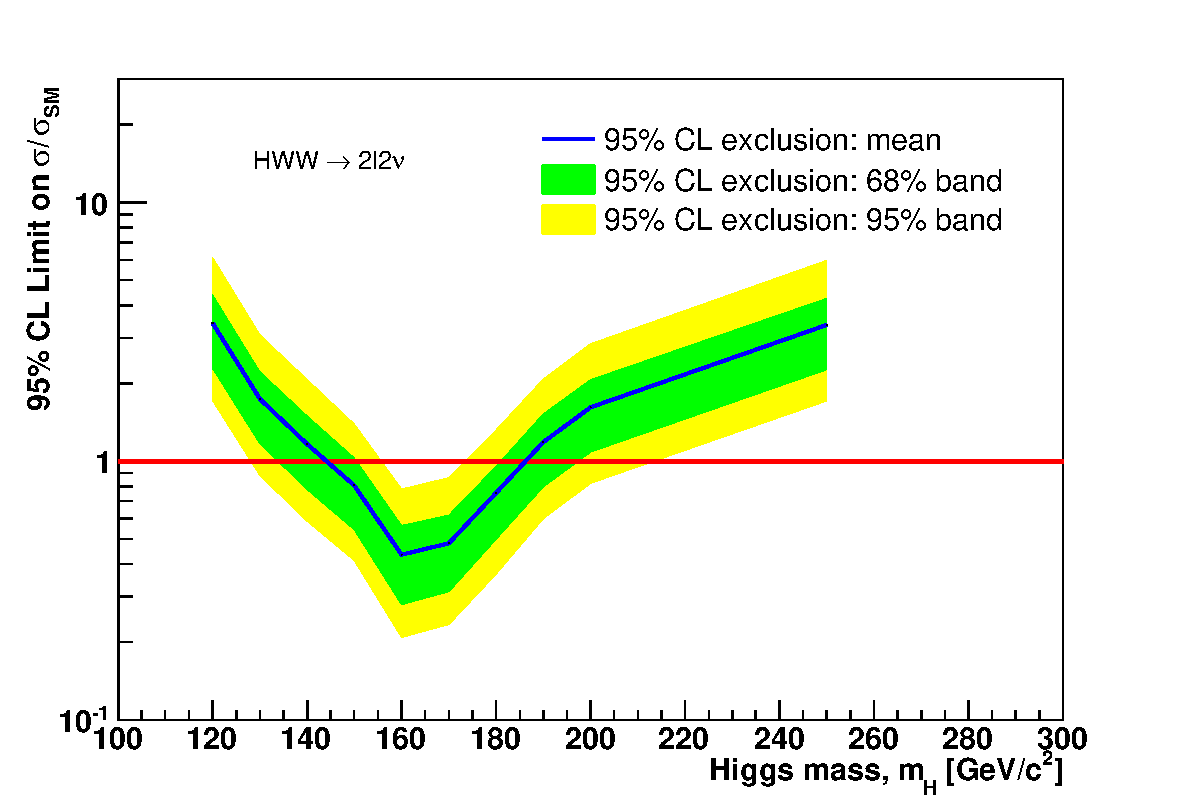
\includegraphics[width=0.9\textwidth]{figures/cut_based_limits.pdf}
   \caption{Cut based analysis expected upper limits at 95\%C.L. for 1\ifb\ of data.}
   \label{fig:cutbase_uls}
\end{center}
\end{figure}


\section{Summary}
    \label{sec:summary}
%    In summary, we described an analysis to study the spin of a single narrow 
resonance at 125 GeV by the gluon fusion through the decays into $WW\to 2\ell2\nu$.  
The analysis is based on a two-dimensional templates $m_T-m_{\ell\ell}$. 
The expected sensitivity to distinguish between between SM Higgs hypothesis and 
spin 2 Graviton like resonance with minimal coupling 
$2_\text{min}^+$ is $1.7\sigma$ for \intlumiEightTeV. 
Scaling by luminosity the projected separation is about $2.0\sigma$ for 25~$\ifb$. 


\clearpage



\appendix
\appendixpage
  \section{Electron Selection Optimization}
     \label{app:els}
     \subsection{Introduction}
The published $H\rightarrow WW\rightarrow 2\ell 2\nu$ analysis of 2010 was based on the following electron selection:
\begin{itemize}
\item identification: VBTF80;
\item isolation: relIso$<$0.10, where relIso is the sum of contributions from tracks, ECAL, and HCAL in a cone of R=0.3 around the electron, 
divided by the electron $p_T$; in the barrel the ECAL contribution has a pedestal subtraction of 1 GeV;
\item impact parameter: transverse longitudinal parameter w.r.t. the primary vertex $<0.02$ cm and longitudinal i.p. $<$ 0.2 cm;
\item conversion rejection: 0 missing inner expected hits and partner track veto (distance $<$0.02 cm, $\Delta \cot \theta <$0.02).
\end{itemize}
Before the 2011 data taking we wanted to review the selection and check if there is anything better available.

This process is divided into two steps: we review the available selections for high $p_T$ electrons ($>$20 GeV) and then, 
we look for improvement for a possible extension at low $p_T$.

The choice of the optimal selection is based on the analysis results after all cuts, 
but we cross-check the performance in terms of efficiency of fake vs good electrons.
Also, we checked the performance in 2011 data and with high PU conditions.

\subsection{Procedure Definition}
The performance of the tested algorithms are evaluated using three figures of merit (FOM):
\begin{itemize}
\item FOM1: $S/B$, the signal to background ratio;
\item FOM2: $S/\sqrt{S+B}$, the statistical significance;
\item FOM3: $S/\sqrt{S+B+(0.35 \cdot B)^2}$, the significance including a 35\% systematic uncertainty on the background;
\end{itemize}
where S and B are the total signal and background yields for an integrated luminosity of 1/fb and evaluated in the 2010 
$H\rightarrow WW\rightarrow 2\ell 2\nu$, $m_H=130$ GeV analysis signal region:
$\Delta\phi < 60$, 12$< m_{ll} <$45 GeV, projected Met$>$35 GeV (20 GeV for $\mu$-e final state), jet and top veto.
In this exercise we consider the final states where the trailing lepton is an electron ($\mu$-e and e-e).
The choice of 35\% in the FOM3 definition is somewhat arbitrary; the idea is to pick a conservative value on the background systematic uncertainty, 
as opposed to FOM2 where the assumption of negligible systematic uncertainty is too optimistic.

Yields are evaluated according to a simple model that treats good and fake electrons separately.
Real electrons are well modeled by simulation and thus we can rely on efficiency estimates from Monte Carlo; 
we use the electron efficiency from the signal sample to scale the signal and non-fake background yields.
Fake and non-prompt electrons, instead, can't be studied on simulation since their physics origin is difficult to parametrize and because
the available sample has low statistics. 
Therefore, we predict the fake background yield from data with the following procedure: 
first, we take as baseline the prediction from 2010 data scaled to 1/fb (using the fake rate method for 2010 analysis electron selection); 
then for each of the tested selections, we calculate the efficiency per fake electron from data and use this efficiency to scale the baseline prediction.

Fake electrons from data are selected from the EG2010A sample requiring HLT\_Ele10\_SW\_L1R and rejecting electrons from W and Z with the following cuts:
Met$<$20 GeV, $m_T(e, Met)<$20 GeV and, for event with two electrons, $|m_{ee}-m_Z|>$15 GeV. 
The selected sample includes about 6500 electrons passing the 2010 analysis selection.

Yields and efficiencies are computed in three bins both in $p_T$ ($[10,15],[15,20],[20,\infty]$, values in GeV) 
and in $|\eta|$ ($[0,1.0],[1.0,1.5],[1.5,2.5]$). 
Tables~\ref{tab:fakeBaseline}-\ref{tab:hww130yieds} report the baseline prediction from 2010 fake data and non-fake background and signal from MC.
For 10$<p_T<$15 GeV the background contribution from fakes is dominant, while at higher $p_T$ it is comparable or smaller than the sum of the other backgrounds.

\begin{table}[!ht]
\begin{center}
\begin{tabular}{|c|ccc|c|} \hline
 & $0.0<|\eta|<1.0$ & $1.0<|\eta|<1.5$ & $1.5<|\eta|<2.5$ & All $\eta$ \\ \hline
10$<p_T<$15 & 9.11 & 3.41 & 1.18 & 13.70 \\
15$<p_T<$20 & 3.22 & 0.00 & 0.93 & 4.15 \\
$p_T>$20 & 1.24 & 2.85 & 1.05 & 5.14 \\  \hline
All $p_T$ & 13.57 & 6.26 & 3.16 & 22.99 \\ \hline
\end{tabular}
\caption{Fake rate prediction for $\mu$-e and e-e final states from 2010 data. 
The electron selection is the same as in 2010 analysis and the results is scaled to 1/fb.
The total uncertainty is of the order of 50\%.
\label{tab:fakeBaseline}}
\end{center}
\end{table}

\begin{table}[!ht]
\begin{center}
\begin{tabular}{|c|ccc|c|} \hline
 & $0.0<|\eta|<1.0$ & $1.0<|\eta|<1.5$ & $1.5<|\eta|<2.5$ & All $\eta$ \\ \hline
10$<p_T<$15 & 2.15 & 0.81 & 1.03 & 4.00 \\
15$<p_T<$20 & 4.18 & 1.42 & 1.26 & 6.87 \\
$p_T>$20    & 10.26& 4.89 & 3.57 & 18.71\\  \hline
All $p_T$   & 16.59& 7.12 & 5.86 & 29.58 \\ \hline
\end{tabular}
\caption{MC yield prediction for non-fake electron backgrounds ($\mu$-e and e-e final states). 
The electron selection is the same as in 2010 analysis and the results is scaled to 1/fb.
\label{tab:nonfakeyieds}}
\end{center}
\end{table}

\begin{table}[!ht]
\begin{center}
\begin{tabular}{|c|ccc|c|} \hline
 & $0.0<|\eta|<1.0$ & $1.0<|\eta|<1.5$ & $1.5<|\eta|<2.5$ & All $\eta$ \\ \hline
10$<p_T<$15 & 0.79 & 0.22 & 0.18 & 1.19 \\
15$<p_T<$20 & 1.09 & 0.37 & 0.32 & 1.78 \\
$p_T>$20    & 2.18 & 0.69 & 0.54 & 3.41 \\  \hline
All $p_T$   & 4.06 & 1.28 & 1.04 & 6.38 \\ \hline
\end{tabular}
\caption{MC yield prediction for $H\rightarrow WW$ sample ($m_H=130$ GeV) ($\mu$-e and e-e final states). 
The electron selection is the same as in 2010 analysis and the results is scaled to 1/fb.
\label{tab:hww130yieds}}
\end{center}
\end{table}

We optimize the electron identification, isolation and impact parameter selections separately, changing one cut at a time.
We checked that, using different isolation algorithms as baseline, the optimal identification working point is the same.
Therefore, we use the 2010 selection as a baseline for the optimization process.

\subsection{Electron Identification}

We compared the performance of several electron identification algorithms available in the collaboration.
They can be grouped in three sets:
\begin{itemize}
\item Simple Cuts (VBTF: 4 variables, separate cuts for barrel/endcap): 
  \begin{itemize}
  \item VBTF85
  \item VBTF80 
  \item VBTF70
  \end{itemize}
\item Multivariate techniques, exploiting correlations between variables (MVA): 
  \begin{itemize}
  \item MVA05: particle flow MVA output$>$0.5 
  \item MVA07: particle flow MVA output$>$0.7 
  \item LHT: Likelihood ID, tight WP\footnote{UserCode/emanuele/EgammaAnalysisTools, tag ``edm-Feb2011'' and latest PDFs: \\
http://indico.cern.ch/getFile.py/access?contribId=4\&resId=0\&materialId=slides\&confId=127254.}
  \end{itemize}
\item Categorized cuts (CIC: advanced cut based tuning in multiple categories)\footnote{CIC version V06 with data driven tuning \\
http://cmssw.cvs.cern.ch/cgi-bin/cmssw.cgi/CMSSW/RecoEgamma/ElectronIdentification/python/\\
cutsInCategoriesElectronIdentificationV06\_DataTuning\_cfi.py?view=log.}: 
  \begin{itemize}
  \item CICST: CIC SuperTight ID 
  \item CICHT2: CIC HyperTight v2 ID
  \item CICHT4: CIC HyperTight v4 ID
  \end{itemize}
\end{itemize}

\subsubsection{Results for $p_T>$20 $\GeVc$}

The first step is the definition of a baseline cut at high $p_T$. 
We verify the identification performance by comparing the cut efficiency on fake electrons from data and on signal electrons on MC.
Figure~\ref{subfig:idEffic_gt20} shows that the MVA curve has worse rejection power than CIC, while the VBTF and CIC curves cross.
This result can be interpreted in terms of analysis performance by looking at the FOM's for $p_{T,max}>$20 GeV and $p_{T,min}>$20 GeV
(Figs.~\ref{subfig:id_hww130_fom1_pt20}-\ref{subfig:id_hww130_fom3_pt20}). 
No algorithm provides the best results for all FOM's; however, it is clear that MVA is slightly worse, while VBTF and CIC are comparable.
Therefore, we think that it is safe to continue with the VBTF approach as baseline for the analysis:
reasonable working points for the $m_H=$130 GeV analysis are VBTF80 and VBTF70. 
However, VBTF70 might be too tight for mass values higher than $m_H=$130 GeV where the $p_T$ spectrum of the signal leptons 
is harder and the fake background less important.
 
\begin{figure}[!hbtp]
\subfigure[]{
\centering
\label{subfig:idEffic_gt20}
\includegraphics[width=.45\textwidth]{figures/idEffic_gt20.png}}
\subfigure[]{
\centering
\label{subfig:id_hww130_fom1_pt20}
\includegraphics[width=.45\textwidth]{figures/id_hww130_fom1_pt20.png}}\\
\subfigure[]{
\centering
\label{subfig:id_hww130_fom2_pt20}
\includegraphics[width=.45\textwidth]{figures/id_hww130_fom2_pt20.png}}
\subfigure[]{
\centering
\label{subfig:id_hww130_fom3_pt20}
\includegraphics[width=.45\textwidth]{figures/id_hww130_fom3_pt20.png}}\\
\caption{Relative ID efficiency (w.r.t. VBTF80) on fake electrons from data vs good electrons from signal MC \subref{subfig:idEffic_gt20};
FOM1, FOM2 and FOM3 \subref{subfig:id_hww130_fom1_pt20},\subref{subfig:id_hww130_fom2_pt20},\subref{subfig:id_hww130_fom3_pt20}. 
Electrons have $p_T>$20 GeV; the 2010 selection is used as a baseline, the ID cut is varied only.}
\label{fig:idpt20}
\end{figure}

\subsubsection{Additional Requirements for $p_T<$20 $\GeVc$}

The cut based approach is a reasonable choice as a baseline for high $p_T$, but at low $p_T$ fakes dominate and more rejection power might be needed; 
Therefore, we propose an additional cut to tighten the selection at low $p_T$.

The idea is to introduce a simple categorization based on fbrem, $\eta$ and $E/p$ (Figure~\ref{fig:smurfcuts}).
When a particle passing electron ID criteria has a high fbrem (fbrem$>$0.15) we are confident it is an electron and we keep it.
Because of the high tracker material budget, at $|\eta|>$1 almost all signal electron radiate and thus we reject all electron candidates with fbrem$<$0.15.
At $|\eta|<$1, instead, there is less tracker material and electrons with low fbrem are frequent: in this region we keep electrons with $E/p>$0.95.

In summary, we apply the following additional cut for electrons with $p_T<$20 GeV:
\begin{equation}
fbrem>0.15~OR~(|\eta|<1~AND~E/p>0.95)
\end{equation}
In the following, we call VBTF80+ (VBTF70+) the VBTF80 (VBTF70) selection added of the proposed cut above.

\begin{figure}[!hbtp]
\subfigure[]{
\centering
\label{subfig:Data_fbrem_eta}
\includegraphics[width=.45\textwidth]{figures/Data_fbrem_eta.png}}
\subfigure[]{
\centering
\label{subfig:Data_eOverPIn_bar}
\includegraphics[width=.45\textwidth]{figures/Data_eOverPIn_bar.png}}\\
\subfigure[]{
\centering
\label{subfig:HWW130_fbrem_eta}
\includegraphics[width=.45\textwidth]{figures/HWW130_fbrem_eta.png}}
\subfigure[]{
\centering
\label{subfig:HWW130_eOverPIn_bar}
\includegraphics[width=.45\textwidth]{figures/HWW130_eOverPIn_bar.png}}\\
\caption{fbrem vs $|\eta|$ (left) and $E/p$ (right) distributions for fake electrons in data (up) and good electrons in signal MC (down).}
\label{fig:smurfcuts}
\end{figure}

\subsubsection{Results for 15$<p_T<$20 $\GeVc$}

The efficiency plot (Figure~\ref{subfig:idEffic_15pt20}) shows that, also in this $p_T$ range, the CIC curve is better than MVA and
the VBTF curve again goes across. It is worth noting that the kink in the last two points of the VBTF curve is due to the additional cuts.
The FOM's for $p_{T,max}>$20 GeV and $p_{T,min}>$15 GeV are shown in Figs.~\ref{subfig:id_hww130_fom1_pt15}-\ref{subfig:id_hww130_fom3_pt15}:
all FOM's are improved w.r.t. to the corresponding values for $p_{T,min}>$20 GeV and an additional improvement is gained using VBTF+.

\begin{figure}[!hbtp]
\subfigure[]{
\centering
\label{subfig:idEffic_15pt20}
\includegraphics[width=.45\textwidth]{figures/idEffic_15pt20.png}}
\subfigure[]{
\centering
\label{subfig:id_hww130_fom1_pt15}
\includegraphics[width=.45\textwidth]{figures/id_hww130_fom1_pt15.png}}\\
\subfigure[]{
\centering
\label{subfig:id_hww130_fom2_pt15}
\includegraphics[width=.45\textwidth]{figures/id_hww130_fom2_pt15.png}}
\subfigure[]{
\centering
\label{subfig:id_hww130_fom3_pt15}
\includegraphics[width=.45\textwidth]{figures/id_hww130_fom3_pt15.png}}\\
\caption{Relative ID efficiency (w.r.t. VBTF80) on fake electrons from data vs good electrons from signal MC \subref{subfig:idEffic_15pt20} 
(15$<p_T<$20 GeV);
FOM1, FOM2 and FOM3 \subref{subfig:id_hww130_fom1_pt15},\subref{subfig:id_hww130_fom2_pt15},\subref{subfig:id_hww130_fom3_pt15} for analysis with  
$p_{T,min}>$15 GeV; the 2010 selection is used as a baseline, the ID cut is varied only.}
\label{fig:idpt15}
\end{figure}

\subsubsection{Results for 10$<p_T<$15 $\GeVc$}

Again, the VBTF+ cuts significantly improve the ID performance (Figure~\ref{subfig:idEffic_10pt15}).
However, despite VBTF+ brings a large relative improvement, the FOM's for $p_{T,max}>$20 GeV and $p_{T,min}>$10 GeV 
(Figs.~\ref{subfig:id_hww130_fom1_pt10}-\ref{subfig:id_hww130_fom3_pt10}) do not show an overall enhancement w.r.t. $p_{T,min}>$15 GeV.

\begin{figure}[!hbtp]
\subfigure[]{
\centering
\label{subfig:idEffic_10pt15}
\includegraphics[width=.45\textwidth]{figures/idEffic_10pt15.png}}
\subfigure[]{
\centering
\label{subfig:id_hww130_fom1_pt10}
\includegraphics[width=.45\textwidth]{figures/id_hww130_fom1_pt10.png}}\\
\subfigure[]{
\centering
\label{subfig:id_hww130_fom2_pt10}
\includegraphics[width=.45\textwidth]{figures/id_hww130_fom2_pt10.png}}
\subfigure[]{
\centering
\label{subfig:id_hww130_fom3_pt10}
\includegraphics[width=.45\textwidth]{figures/id_hww130_fom3_pt10.png}}\\
\caption{Relative ID efficiency (w.r.t. VBTF80) on fake electrons from data vs good electrons from signal MC \subref{subfig:idEffic_10pt15} 
(10$<p_T<$15 GeV);
FOM1, FOM2 and FOM3 \subref{subfig:id_hww130_fom1_pt10},\subref{subfig:id_hww130_fom2_pt10},\subref{subfig:id_hww130_fom3_pt10} for analysis with  
$p_{T,min}>$10 GeV; the 2010 selection is used as a baseline, the ID cut is varied only.}
\label{fig:idpt10}
\end{figure}

\subsubsection{Conclusions}

In summary, the cut based approach for electron ID is optimal for the $H\rightarrow WW$ analysis and the proposed additional cuts add more rejection power 
for $p_T<$20 GeV. Lowering the $p_{T,min}$ cut to 15 GeV improves the analysis, while at 10 GeV there is no clear benefit. 
Thus, we choose VBTF80 for $p_T>$20 GeV and VBTF70+ for 15$<p_T<$20 GeV.

\subsection{Electron Isolation}

The 2010 analysis used relIso$<$0.10.
Given that the ID optimization suggests to lower the  $p_{T,min}$ cut to 15 GeV, we wanted to review if tightening the isolation cut further 
would improve the performance of the analysis.
Within the cut based approach, we can tighten the cut in three ways: lowering the cut value, increasing the cone size, and removing the pedestal subtraction.
In the following tests, we call (tight) sliding isolation the following set of cuts: 
\begin{itemize}
\item relIso$<$0.1 (0.1) for $p_T>$20 GeV
\item relIso$<$0.07 (0.03) for 15$<p_T<$20 GeV
\item relIso$<$0.05 (0.01) for 10$<p_T<$15 GeV
\end{itemize}
and we will test it with cone size 0.3 and cone size 0.4 with and without pedestal subtraction.
CIC isolation uses cone size 0.3 for the tracker and 0.4 for the calorimeters and does not apply pedestal subtracion; cut values are optimized for various categories.
Results are summarized in Figure~\ref{fig:isopt15}. 
The efficiency plot shows that the cut based approach is basically one single curve covering the whole range and it is slightly worse than CIC; 
however, there is not a clear advantage in using tighter isolation approaches since FOM1 and FOM3 slightly improve, while FOM2 worsens. 
Therefore, we choose to stick to the relIso$<$0.10 cut. This exercise will be repeated with 2011 fake data.

\begin{figure}[!hbtp]
\subfigure[]{
\centering
\label{subfig:isoEffic_15pt20}
\includegraphics[width=.45\textwidth]{figures/isoEffic_15pt20.png}}
\subfigure[]{
\centering
\label{subfig:iso_hww130_fom1_pt15}
\includegraphics[width=.45\textwidth]{figures/iso_hww130_fom1_pt15.png}}\\
\subfigure[]{
\centering
\label{subfig:iso_hww130_fom2_pt15}
\includegraphics[width=.45\textwidth]{figures/iso_hww130_fom2_pt15.png}}
\subfigure[]{
\centering
\label{subfig:iso_hww130_fom3_pt15}
\includegraphics[width=.45\textwidth]{figures/iso_hww130_fom3_pt15.png}}\\
\caption{Relative isolation efficiency (w.r.t. relIso) on fake electrons from data vs good electrons from signal MC \subref{subfig:isoEffic_15pt20} 
(15$<p_T<$20 GeV);
FOM1, FOM2 and FOM3 \subref{subfig:iso_hww130_fom1_pt15},\subref{subfig:iso_hww130_fom2_pt15},\subref{subfig:iso_hww130_fom3_pt15} for analysis with  
$p_{T,min}>$15 GeV; the 2010 selection is used as a baseline, the isolation cut is varied only.}
\label{fig:isopt15}
\end{figure}

\subsection{Impact Parameter}

The same test have been performed varying the impact parameter (IP) cut.
We have tested the folowing approaches:
\begin{itemize}
\item 2D impact parameter cut
\item 2D impact parameter significance cut
\item 3D impact parameter cut
\item 3D impact parameter significance cut
\end{itemize}
where the impact parameter is computed with respect to the signal primary vertex (PV) reconstructed with the standard vertexing 
algorithm (\emph{offlinePrimaryVertex}).
Figure~\ref{subfig:ipEffic_15pt20} shows that, for 15$<p_T<$20 the best performance are obtained with the 2D impact parameter plain cut.
The FOM's show very little difference between the various approaches (Figs.~\ref{fig:ippt15}\subref{subfig:ip_hww130_fom1_pt15}-\subref{subfig:ip_hww130_fom3_pt15}).
We choose a 2D impact parameter cut value of 0.02 cm.

\begin{figure}[!hbtp]
\subfigure[]{
\centering
\label{subfig:ipEffic_15pt20}
\includegraphics[width=.45\textwidth]{figures/ipEffic_lt20.png}}
\subfigure[]{
\centering
\label{subfig:ip_hww130_fom1_pt15}
\includegraphics[width=.45\textwidth]{figures/ip_hww130_fom1_pt15.png}}\\
\subfigure[]{
\centering
\label{subfig:ip_hww130_fom2_pt15}
\includegraphics[width=.45\textwidth]{figures/ip_hww130_fom2_pt15.png}}
\subfigure[]{
\centering
\label{subfig:ip_hww130_fom3_pt15}
\includegraphics[width=.45\textwidth]{figures/ip_hww130_fom3_pt15.png}}\\
\caption{Relative IP efficiency (w.r.t. d0(PV)$<$0.02) on fake electrons from data vs good electrons from signal MC \subref{subfig:ipEffic_15pt20} 
(15$<p_T<$20 GeV);
FOM1, FOM2 and FOM3 \subref{subfig:ip_hww130_fom1_pt15},\subref{subfig:ip_hww130_fom2_pt15},\subref{subfig:ip_hww130_fom3_pt15} for analysis with  
$p_{T,min}>$15 GeV; the 2010 selection is used as a baseline, the d0 cut is varied only.}
\label{fig:ippt15}
\end{figure}

\subsection{Studies with Data}

We measured the efficiency of the additional proposed cuts on 2010 data using the tag and probe method.
We use a N-1 approach, where we choose di-electron events with 76$<M_{ee}<$106 GeV and the denominator is given by electrons passing 2010 analysis selection
and the numerator by 2010 selection plus the additional proposed cut. 
Results (Fig.~\ref{fig:eID-tnp}) show that the efficiency on Z electron is at the level of 90\%
or higher and data and MC are in good agreement. The error bars are statistical only.

\begin{figure}[!hbtp]
\centering
\includegraphics[width=.45\textwidth]{figures/eID-tnp.png}
\caption{Efficiency of the additional cut with the tag and probe method on 2010 $Z\rightarrow ee$ data and MC as a function of probe $p_T$.}
\label{fig:eID-tnp}
\end{figure}

We also checked the distribution of the electron ID variables in the first 2011 data and compared it with MC.
We analyzed ExpressStream data, selecting Z events with 76$<M_{ee}<$106 GeV, $p_{T,max}>$27 GeV (so that it passes the single electron trigger), 
$p_{T,min}>$10 GeV, relative isolation$<$0.2 for tracks, ECAL and HCAL separately and $\sigma_{i\eta i\eta}<$0.015 (0.031) for barrel (endcap).
Given that no selection for good run certification is applied, all distributions (Figs.~\ref{fig:mcdata_vbtf_bar}-\ref{fig:mcdata_smurf}) 
are in reasonable agreement except $H/E$ in the endcap (Fig.~\ref{subfig:mcdata_hOverE_end_log}). 
As other studies on high pile-up samples confirm, this variable is particularly sensitive to the pile-up conditions and can introduce data-MC discrepancies 
in the electron identification efficiency up to the 20\% level at large $|\eta|$.
We verified that with our current selection (VBTF80 for $p_T>$20 GeV and VBTF70+ for 15$<p_T<$20 GeV) we can remove the $H/E$ cut in the endcap
region without significant decrease in the analysis performance (Fig.~\ref{fig:idpt15_nohoe}). We define as VBTF- the VBTF identification without the $H/E$ cut in the endcap.

\begin{figure}[!hbtp]
\subfigure[]{
\centering
\label{subfig:mcdata_dPhiIn_bar_log}
\includegraphics[width=.45\textwidth]{figures/mcdata_dPhiIn_bar_log.png}}
\subfigure[]{
\centering
\label{subfig:mcdata_dEtaIn_bar_log}
\includegraphics[width=.45\textwidth]{figures/mcdata_dEtaIn_bar_log.png}}\\
\subfigure[]{
\centering
\label{subfig:mcdata_sigmaIEtaIEta_bar_log}
\includegraphics[width=.45\textwidth]{figures/mcdata_sigmaIEtaIEta_bar_log.png}}
\subfigure[]{
\centering
\label{subfig:mcdata_hOverE_bar_log}
\includegraphics[width=.45\textwidth]{figures/mcdata_hOverE_bar_log.png}}\\
\caption{VBTF electron ID variables (barrel) in MC and in early 2011 data. Distributions are normalized to the number of entries in data.}
\label{fig:mcdata_vbtf_bar}
\end{figure}

\begin{figure}[!hbtp]
\subfigure[]{
\centering
\label{subfig:mcdata_dPhiIn_end_log}
\includegraphics[width=.45\textwidth]{figures/mcdata_dPhiIn_end_log.png}}
\subfigure[]{
\centering
\label{subfig:mcdata_dEtaIn_end_log}
\includegraphics[width=.45\textwidth]{figures/mcdata_dEtaIn_end_log.png}}\\
\subfigure[]{
\centering
\label{subfig:mcdata_sigmaIEtaIEta_end_log}
\includegraphics[width=.45\textwidth]{figures/mcdata_sigmaIEtaIEta_end_log.png}}
\subfigure[]{
\centering
\label{subfig:mcdata_hOverE_end_log}
\includegraphics[width=.45\textwidth]{figures/mcdata_hOverE_end_log.png}}\\
\caption{VBTF electron ID variables (endcap) in MC and in early 2011 data. Distributions are normalized to the number of entries in data.}
\label{fig:mcdata_vbtf_end}
\end{figure}


\begin{figure}[!hbtp]
\subfigure[]{
\centering
\label{subfig:mcdata_fbrem_bar1_log}
\includegraphics[width=.45\textwidth]{figures/mcdata_fbrem_bar1_log.png}}
\subfigure[]{
\centering
\label{subfig:mcdata_fbrem_end1_log}
\includegraphics[width=.45\textwidth]{figures/mcdata_fbrem_end1_log.png}}\\
\subfigure[]{
\centering
\label{subfig:mcdata_eOverPIn_bar1_log}
\includegraphics[width=.45\textwidth]{figures/mcdata_eOverPIn_bar1_log.png}}
\caption{VBTF+ additional electron ID variables in MC and in early 2011 data. Distributions are normalized to the number of entries in data.}
\label{fig:mcdata_smurf}
\end{figure}

\begin{figure}[!hbtp]
\subfigure[]{
\centering
\label{subfig:idEffic_15pt20_nohoe}
\includegraphics[width=.45\textwidth]{figures/idEffic_15pt20_nohoe.png}}
\subfigure[]{
\centering
\label{subfig:id_hww130_fom1_pt15_nohoe}
\includegraphics[width=.45\textwidth]{figures/id_hww130_fom1_pt15_nohoe.png}}\\
\subfigure[]{
\centering
\label{subfig:id_hww130_fom2_pt15_nohoe}
\includegraphics[width=.45\textwidth]{figures/id_hww130_fom2_pt15_nohoe.png}}
\subfigure[]{
\centering
\label{subfig:id_hww130_fom3_pt15_nohoe}
\includegraphics[width=.45\textwidth]{figures/id_hww130_fom3_pt15_nohoe.png}}\\
\caption{Relative ID efficiency for (w.r.t. VBTF80) on fake electrons from data vs good electrons from signal MC including VBTF- \subref{subfig:idEffic_15pt20_nohoe} 
(15$<p_T<$20 GeV);
FOM1, FOM2 and FOM3 \subref{subfig:id_hww130_fom1_pt15_nohoe},\subref{subfig:id_hww130_fom2_pt15_nohoe},\subref{subfig:id_hww130_fom3_pt15_nohoe} for analysis with  
$p_{T,min}>$15 GeV; the 2010 selection is used as a baseline, the ID cut is varied comparing VBTF with VBTF-.}
\label{fig:idpt15_nohoe}
\end{figure}

\subsection{Conclusion}
After the optimization procedure and the tests on data we define the following electron selection for 2011 $H\rightarrow WW$ analysis (conversion rejection not included here, it was optimized with a different procedure):
\begin{itemize}
\item identification: 
  \begin{itemize}
  \item 15$<$pt$<$20: VBTF70 (no H/E cut for endcap) AND (fbrem$>$0.15 OR ($|\eta|<$1 AND E/p$>$0.95)
  \item pt$>$20: VBTF80 (no H/E cut for endcap)
  \end{itemize}
\item isolation: relIso$<$0.10, where relIso is the sum of contributions from tracks, ECAL and HCAL is a cone of R=0.3 around the electron, 
  divided by the electron $p_T$; in the barrel the ECAL contribution has a pedestal subtrction of 1 GeV;
\item impact parameter: transverse longitudinal parameter w.r.t. the primary vertex $<0.02$ cm and longitudinal i.p. $<$ 0.2 cm;
\end{itemize}

  \section{Muon Selection Optimization}
     \label{app:mus}
     \section{Muon ID}

To increase sensitivity to a lower mass Higgs boson, the lepton $p_T$ threshold needs to be lowered. However, background contributions from muon fakes occur more often at lower momenta. The selection requirements from AN-10-344 were optimized for leptons above $20\:\GeVoverc$. This section presents studies on isolation and impact parameter requirements to improve the muon identification performance in the range, $10\:\GeVoverc < p_T < 20\:\GeVoverc$.

The nominal selection is extended to allow for one lepton with $p_T$ down to $10\:\GeVoverc$. The expected yield in $1\:\invfb$ is computed by applying the selection to the Higgs signal sample for mass $130\:\GeVovercsq$ and to all Monte Carlo background samples except $W+$jets. The $W+$jets expectation is derived by applying the fake rate method on the $W+$jets Monte Carlo sample and the details are explained in a later sub-section. The reason for the unique treatment of $W+$jets is because too few events remain after applying selection on the $W+$jets Monte Carlo, and too few tight-loose candidates are found in data to make a useful extrapolation. The nominal yield expectations for the $e\mu$ and $\mu\mu$ final states are listed in Table~\ref{tab:muidyield0}, where the trailing lepton is a muon.

\begin{table}[!htbp]
\begin{center}
\begin{tabular}{|l|c|c|c|}
\hline
	Source & $p_T > 20$ & $15 < p_T < 20$ & $10 < p_T < 15$ \\
\hline
$H\rightarrow WW$ ($e\mu$) & $2.428$  & $1.587$ & $1.305$ \\
$W+$jets ($e+$fake $\mu$)  & $0$      & $0.77$  & $2.64$ \\
Other backgrounds($e\mu$)  & $12.167$ & $6.325$ & $4.161$ \\
\hline
$H\rightarrow WW$ ($\mu\mu$) & $2.553$  & $1.399$ & $1.047$ \\
$W+$jets ($\mu$+fake $\mu$)  & $0.11$   & $1.94$  & $1.20$ \\
Other backgrounds($\mu\mu$)  & $13.664$ & $7.576$ & $3.647$ \\
\hline
\end{tabular}
\caption{Predicted yields for $1\:\invfb$ in the $e\mu$ and $\mu\mu$ final states with the nominal selection extended to allow a lepton leg down to $10\:\GeVoverc$.}
\label{tab:muidyield0}
\end{center}
\end{table}

\subsection{Fake Rate Method}
The fake rate method is applied for two purposes in this study. As discussed above, the method is applied to the $W+$jets Monte Carlo sample to extract a yield for lepton plus muon fake events. The method is also applied to the data to determine how the fake rate varies with changing the isolation and impact parameter requirements. The relative change of the fake rate in data is then used to re-scale the Monte Carlo prediction.

The fakeable object is defined as a GlobalMuon satisfying,
\begin{itemize}
\item TrackerMuon reconstruction,
\item at least $11$ tracker hits,
\item global fit $\chi^2/$NDF $< 10$,
\item at least $1$ valid muon hit in the global fit,
\item $(I_{trk}+I_{ECAL}+I_{HCAL})/p_T < 1$,
\item $d_0 < 0.2\:$cm with respect to the primary vertex.
\end{itemize}
The event primary vertex is the reconstructed vertex with the highest $\sum p_T^2$ using the Deterministc Annealing algorithm and satisfying standard quality cuts.

In the $W+$jets Monte Carlo, the fakeable object is required to not be within $\Delta R<0.5$ of the generator level muon in the cases of a $W\rightarrow\mu\nu$ event or a $W\rightarrow\tau\nu$ event where the tau decays to a muon, nor be within $\Delta R<0.5$ of the generator level tau in the case of a $W\rightarrow\tau\nu$ event where the tau decays hadronically.

In data, the fakeable object selection must ensure minimal contamination by prompt muons from $W$ and $Z$ decays. The following cuts are applied,
\begin{itemize}
\item $Z$ veto: event is rejected if there are two oppositely charged muons with $p_T>20\:\GeVoverc$ satisfying the fakeable object definition, 
\item $W$ veto: event is rejected if PF-MET $> 20\:\GeV$ or the muon has transverse mass larger than $20\:\GeVovercsq$,
\item there is a PF-jet away from the fakeable object ($\Delta R > 1$) with $p_T>15\:\GeVoverc$ after L2-Relative, L3-Absolute, L2L3-Residual jet corrections and energy density subtraction from the FastJet technique.
\end{itemize}
The motivation for the final criteria listed above is to select events that emulate $W+$jets conditions. The fake rate calibration in data was performed on $5\invpb$ of 2011 data.

\subsection{Figures Of Merit}
As Table~\ref{tab:muidyield0} shows, the background contribution from fakes is not dominant even with the lowered muon $p_T$ requirement. Hence, when tuning the selection cuts on isolation and impact parameter, the objective should not be to reject fakes as much as possible. The performance of the selection criteria is quantified by several figures of merit (FOMs), 
\begin{itemize}
\item $S/B$
\item $S/\sqrt{S+B}$
\item $S/\sqrt{S+B+(\sigma B)^2}$, where $\sigma=0.35$ is the background systematic uncertainty.
\end{itemize}
The FOMs for the nominal selection for the ``20-20'' $p_T$ cuts and for the ``20-10'' $p_T$ cuts are listed in Table~\ref{tab:muidfom0}. It can be seen that just by lowering the $p_T$ threshold, we gain more signal events and we get a substantial increase in the FOMs except for $S/B$. We proceed to study isolation and impact parameter to find an improved working point.

\begin{table}[!htbp]
\begin{center}
\begin{tabular}{|l|c|c|c|}
\hline
	``20-20'' cuts & $e\mu$ & $\mu\mu$ & Both \\
\hline
$S/B$                       & $0.20$ & $0.19$ & $0.19$ \\
$S/\sqrt{S+B}$              & $0.64$ & $0.63$ & $0.90$ \\
$S/\sqrt{S+B+(\sigma B)^2}$ & $0.42$ & $0.41$ & $0.47$ \\
\hline\hline
	``20-10'' cuts & $e\mu$ & $\mu\mu$ & Both \\
\hline
$S/B$                       & $0.20$ & $0.18$ & $0.19$ \\
$S/\sqrt{S+B}$              & $0.95$ & $0.87$ & $1.29$ \\
$S/\sqrt{S+B+(\sigma B)^2}$ & $0.50$ & $0.44$ & $0.50$ \\
\hline
\end{tabular}
\caption{FOMs for the ``20-20'' and ``20-10'' selection using muon identification criteria of AN-10-344.}
\label{tab:muidfom0}
\end{center}
\end{table}

\subsection{Isolation}
We consider varying the isolation cut from the nominal value of $0.15$ down to $0.05$. The curves of fake rate versus signal muon efficiency are shown in Figure~\ref{fig:isoscan}. The signal muon efficiency here is defined as the efficiency to pass full selection, with the modified isolation cut, with respect to a reconstructed muon passing the fakeable object requirements and matched to the generator level muon from $H\rightarrow WW$.

\begin{figure}[!htbp]
\begin{center}
\includegraphics[scale=0.4]{figures/isoscan0.eps}
\includegraphics[scale=0.4]{figures/isoscan1.eps}
\includegraphics[scale=0.4]{figures/isoscan2.eps}
\caption{Fake rates versus signal muon efficiency for varying isolation cut in different $p_T$ bins.}
\label{fig:isoscan}
\end{center}
\end{figure}

The corresponding FOMs are shown in Figure~\ref{fig:isofoms}. Taking the FOMs and signal muon efficiencies into consideration, we choose a working point of $I<0.10$ for muons in the $10\:\GeVoverc < p_T < 20\:\GeVoverc$ range.
\begin{figure}[!htbp]
\begin{center}
\includegraphics[scale=0.55]{figures/iso_fom1.eps}
\includegraphics[scale=0.55]{figures/iso_fom2.eps}
\includegraphics[scale=0.55]{figures/iso_fom3.eps}
\caption{Figures of merit for varying isolation cut.}
\label{fig:isofoms}
\end{center}
\end{figure}

\subsection{Impact Parameter}
We consider varying the impact parameter cut from the nominal value of $0.020\:$cm down to $0.005\:$cm. The curves of fake rate versus signal muon efficiency are shown in Figure~\ref{fig:ipscan}. It can be seen that $d_0$ and $d_0$-significance give very similar performance, so we decide to stay with using the $d_0$ variable as used in AN-10-344.

\begin{figure}[!htbp]
\begin{center}
\includegraphics[scale=0.4]{figures/ipscan0.eps}
\includegraphics[scale=0.4]{figures/ipscan1.eps}
\includegraphics[scale=0.4]{figures/ipscan2.eps}
\caption{Fake rates versus signal muon efficiency for varying impact parameter cut in different $p_T$ bins.}
\label{fig:ipscan}
\end{center}
\end{figure}

The corresponding FOMs are shown in Figure~\ref{fig:ipfoms}. We choose a working point of $d_0<0.01\:$cm for muons in the $10\:\GeVoverc < p_T < 20\:\GeVoverc$ range.
\begin{figure}[!htbp]
\begin{center}
\includegraphics[scale=0.55]{figures/d0_fom1.eps}
\includegraphics[scale=0.55]{figures/d0_fom2.eps}
\includegraphics[scale=0.55]{figures/d0_fom3.eps}
\caption{Figures of merit for varying $d_0$ cut.}
\label{fig:ipfoms}
\end{center}
\end{figure}

\subsection{Results}
A summary of FOMs is provided in Table~\ref{tab:muidfom1}. Our chosen working point gives roughly a $5\%$ improvement in $S/B$ and a $4\%$ improvement in $S/\sqrt{S+B+(\sigma B)^2}$, while $S/\sqrt{S+B}$ suggests the performance degrades by about $1\%$.

\begin{table}[!htbp]
\begin{center}
\begin{tabular}{|l|c|c|c|}
\hline
	``20-20'' cuts & $e\mu$ & $\mu\mu$ & Both \\
\hline
$S/B$                       & $0.20$ & $0.19$ & $0.19$ \\
$S/\sqrt{S+B}$              & $0.64$ & $0.63$ & $0.90$ \\
$S/\sqrt{S+B+(\sigma B)^2}$ & $0.42$ & $0.41$ & $0.47$ \\
\hline\hline
	``20-10'' cuts & $e\mu$ & $\mu\mu$ & Both \\
\hline
$S/B$                       & $0.20$ & $0.18$ & $0.19$ \\
$S/\sqrt{S+B}$              & $0.95$ & $0.87$ & $1.29$ \\
$S/\sqrt{S+B+(\sigma B)^2}$ & $0.50$ & $0.44$ & $0.50$ \\
\hline\hline
	tight cuts & $e\mu$ & $\mu\mu$ & Both \\
\hline
$S/B$                       & $0.21$ & $0.19$ & $0.20$ \\
$S/\sqrt{S+B}$              & $0.94$ & $0.86$ & $1.27$ \\
$S/\sqrt{S+B+(\sigma B)^2}$ & $0.51$ & $0.45$ & $0.52$ \\
\hline
\end{tabular}
\caption{Summary of FOMs for the nominal cuts from AN-10-344 and our chosen working point.}
\label{tab:muidfom1}
\end{center}
\end{table}

The fake rate in the 2011 data before and after our chosen working point is shown in Figure~\ref{fig:mufakerate0}. The fake rate in bins of reconstructed vertices are shown in Figure~\ref{fig:mufakerate1}. The counted vertices are simply required to be valid and not fake. There is no apparent dependence of the fake rate on pile-up.

\begin{figure}[!htbp]
\begin{center}
\includegraphics[scale=0.33]{figures/frpt_old.eps}
\includegraphics[scale=0.33]{figures/frpt_new.eps} \\
\includegraphics[scale=0.33]{figures/freta_old.eps}
\includegraphics[scale=0.33]{figures/freta_new.eps}
\caption{Fake rate projections on $p_T$ (top) and $\eta$ (bottom) for the old muon identification selection (left) and the new selection with tighter isolation and $d_0$ (right).}
\label{fig:mufakerate0}
\end{center}
\end{figure}

\begin{figure}[!htbp]
\begin{center}
\includegraphics[scale=0.5]{figures/frpt_pu.eps}
\includegraphics[scale=0.5]{figures/freta_pu.eps}
\caption{Fake rate projections on $p_T$ and $\eta$ in different bins of reconstructed vertices with the tighter selection.}
\label{fig:mufakerate1}
\end{center}
\end{figure}
  \section{$\met$ Options}
     \label{app:met}
%     \input{appendix_met}

%%   \section{Electron selection details}\label{sec:eledetail}
%%     \input{electron_detail}
%%   \section{Using the transverse mass of the $W$ for
%%     \dytt\ suppression}\label{sec:mt} 
%%     \input{mt}
%%   \section{Jet Veto at high $\eta$}
%%     \input{higheta}
%%   \section{Jet Veto using $b$ tagging}
%%     \input{btagging}
%%   \section{Application of the Drell-Yan estimate method}
%%     \label{app:dy22X}
%%     \input{drell_yan_appendix}
%%   \section{Event yields in other samples}
%%     \label{app:othersamples}
%%     \input{alt_samples}
%%   \section{Estimating the sensitivity to observe \ww\ in 100/pb}
%%     \label{app:significance}
%%     \input{significance}
%%   \section{QCD multi jet background estimation}
%%     \label{app:qcd}
%%     \input{qcd}
%% \clearpage

\vspace*{-0.2cm}
\thebibliography{12}

\bibitem{pdg}
 K. Nakamura et al. (Particle Data Group), "Review of particle physics", J. Phys.G37 , 2010.

\bibitem{Higgs1}
F. Englert and R. Brout, "Broken symmetries and the masses of gauge bosons", Phys. Rev. Lett. 13,  1964.

\bibitem{Higgs2}
P. W. Higgs, "Broken symmetry and the mass of gauge vector mesons", Phys. Rev. Lett. 13, 1964.

\bibitem{Higgs3}
Guralnik, G.S. and Hagen, C.R. and Kibble, T.W.B., "Global Conservation Laws and Massless Particles", 
Phys.Rev.Lett. 13, 1964.

\bibitem{HWW2010}
CMS Collaboration, "Title: Measurement of WW Production and Search for the Higgs Boson in 
pp Collisions at $\sqrt{s}$ = 7 TeV", arXiv:1102.5429

\bibitem{VBTFCrossSectionNote}
J. Alcaraz Maestre, \textit{et al.}, "Updated Measurements of Inclusive W and Z Cross Sections 
at $\sqrt{s}=7$ TeV", CMS AN-2010/264.

\bibitem{ggWWError}
F.~ Stoeckli, "http://indico.cern.ch/getFile.py/access?contribId=0\&resId=1\&materialId=slides\&confId=49009", 
EWK Diboson meeting of March 12 2009.

\bibitem{json}
{\small
/afs/cern.ch/cms/CAF/CMSCOMM/COMM\_DQM/certification/Collisions11/7TeV/Prompt/Cert\_160404-163869\_7TeV\_PromptReco\_Collisions11\_JSON.txt
}

\bibitem{ElIso}
A. Vartak, M. LeBourgeois, V. Sharma, "Lepton Isolation in the CMS Tracker, ECAL and HCAL", CMS AN-2010/106.

\bibitem{PVDA}
W. Erdmann, M. LeBourgeois, B. Mangano, 
https://indico.cern.ch/getFile.py/access?contribId=5\&sessionId=3\&resId=1\&materialId=slides\&confId=127127, 
note in preparation.

\bibitem{NExpHits}
B. Mangano \textit{et al.}, "Improvement in Photon Conversion Rejection Performance Using 
Advanced Tracking Tools", AN-10-283.

\bibitem{fakeLeptonNote1}
S.~Xie, \textit{et al.}", "Study of Data-Driven Methods for Estimation of Fake Lepton Backgrounds", 
CMS AN-2009/120.

\bibitem{fakeLeptonNote2}
W.~Andrews, \textit{et al.}, "Fake Rates for dilepton Analyses", CMS AN-2010/257.

\bibitem{fakeLeptonBkgSpillage1}
 F. Golf, D. Evans, J. Mulmenstadt  \textit{et al.}, ``Expectations for observation of top quark pair production in the dilepton final state with the early CMS data'', CMS AN-2009/050.

\bibitem{dyestnote}
W. Andrews, et al., “A Method to Measure the Contribution of $\dyll$ to a di-lepton+ MET Selection”, CMS AN-2009/023 (2009).

\bibitem{jes}
CMS Collaboration, "Jet Energy Calibration with Photon+Jet Events", PAS JME-09-004.

\bibitem{jetpas}
CMS Collaboration, "Jet Performance in pp Collisions at $\sqrt{s}=7 \rm\ TeV$", PAS JME-10-003.

\bibitem{btag}
CMS collaboration, "Commissioning of b-jet identification with pp collisions at $\sqrt{s}=7~\TeV$, BTV-10-001.

\bibitem{antikt}
Cacciari, Matteo and Salam, Gavin P. and Soyez, Gregory, "The anti-$k_t$ jet clustering 
algorithm", JHEP 04,  2008.

\bibitem{ConversionNote}
W.~Andrews, \textit{et al.}, "Study of photon conversion rejection at CMS", CMS AN-2009/159.

\bibitem{tmva}
A. Hoecker, \textit{et al.}, "TMVA - Toolkit for Multivariate Data Analysis", arXiv:physics/0703039, 2007.

\bibitem{XS}
CMS Generator group, Standard Model Cross Sections for CMS at 7 TeV, 2010.

\bibitem{PDF4LHC}
PDF4LHC Working Group, 
{\tt http://www.hep.ucl.ac.uk/pdf4lhc/PDF4LHCrecom.pdf}

\bibitem{Nadolsky:2008zw}
Nadolsky, Pavel M. and others, "Implications of CTEQ global analysis for 
collider observables", Phys. Rev. D78 2008.

\bibitem{Martin:2009iq}
Martin, A. D. and Stirling, W. J. and Thorne, R. S. and Watt, G., "Parton 
distributions for the LHC, Eur. Phys. J. C63 2009.

\bibitem{Ball:2010de}
Ball, Richard D. and others, "A first unbiased global NLO determination 
of parton distributions and their uncertainties", arXiv 1002.4407.

\bibitem{bayesian}
A. O'Hagan and J.J. Forster, "Bayesian Inference", Kendall's Advanced Theory of Statistics, 
Arnold, London, 2B, 2004.

\bibitem{ref:tagprobe_mit_w}
G. Bauer {\it et. al.}, "Lepton ef?iencies for the inclusive W cross section measurement with 36.1pb$^{-1}$", AN2011/097

\bibitem{ref:tagprobe_snt_top}
W. Andrews {\it et. al.}, "Uncertainties on the Lepton Selection Efficiency for t$t\bar{t}$ Cross Section Analysis", AN2010/274

\bibitem{LHCHiggsCrossSectionWorkingGroup:2011ti}
LHC Higgs Cross Section Working Group, "Handbook of LHC Higgs Cross Sections: 
Inclusive Observables", CERN-2011-002, 2011.

\bibitem{PFMET} 
CMS Collaboration, ``CMS MET Performance in Events Containing Electroweak Bosons from pp Collisions at $\sqrt{s}=7$ TeV'', CMS PAS JME-2010-005 (2010)


\bibitem{trkMET} 
Marco Zanetti, ``MET with PU in $\hww\to2\ell$'', https://indico.cern.ch/conferenceDisplay.py?confId=131580
Benjamin Hooberman, ``MET with PU in MC and First 2011 Data'', https://indico.cern.ch/contributionDisplay.py?contribId=5\&confId=132579. 


\bibitem{lands}
Mingshui Chen and Andrey Korytov, https://mschen.web.cern.ch/mschen/lands/

\bibitem{MCFMHiggsProduction}
J. Campbell, R.K. Ellis, G. Zanderighi, ``Next-to-Leading order Higgs + 2 jet production via gluon fusion.'', JHEP 0610:028 (2006), hep-ph/0608194

\end{document}
